\chapter{Grundlagen}

Ziel dieser Arbeit ist die Ermittlung optimierter Gebäudeenergiesysteme für den deutschen Wohngebäudebestand.
Hierzu wird in Kapitel \ref{sec:Sektion 21} der Bestand analysiert, um auf dieser Untersuchung aufbauend die nationale Wohngebäudesituation in einigen wenigen, repräsentativen Klassen abzubilden. 
Des Weiteren wird in \ref{sec:Sektion 22} die historische Entwicklung der Gebäudehülle im Neubauzustand betrachtet und in \ref{sec:Sektion 23} die Abweichungen des Neubauzustandes durch Sanierung erläutert. Daraus werden Zeiträume der Baualtersklassen mit ähnlichen Baustoffen und Dämmdicken zusammengefasst. 
Kapitel \ref{sec:Sektion 24} stellt Förderprogramme zum Anreiz energetischer Sanierung vor.
Zuletzt stellen Kapitel \ref{sec:Sektion 25} und \ref{sec:Sektion 26} die Grundlagen der mathematischen Optimierung sowie das im Rahmen dieser Arbeit erweiterte Optimierungsprogramm vor. 

%Gebäudeenergiesysteme erklären?
%Was hat das überhaupt mit Grundlagen zu tuen, was ich da schreibe?
%Nehm ich in der Einleitung des Kapitels hier zuviel vorweg?



\section{Deutscher Wohngebäudebestand}
\label{sec:Sektion 21}

Zunächst wird der Wohngebäudebestand hinsichtlich Alter und Größe ausgewertet.
Als Daten werden die Statistiken des Zensus2011, einer nationalen statistischen Erhebung von privaten Haushalten, betrachtet. 
Besagte Statistiken werden in verschiedenen wissenschaftlichen Untersuchungen des Instituts für Wohnen und Umwelt GmbH (IWU) ausgewertet und evaluiert.
Weiterhin werden für die gebäudetypischen Kennwerte die Typgebäude des europaweiten Projekts \glqq Typology Approach for Building Stock Energy Assessment\grqq\,(TABULA) berücksichtigt. Die nationalen Daten Deutschlands wurden durch das IWU erhoben und berechnet.
%Tabula evtl erst im nächsten Kapitel erläutern, da bei der statistischen Betrachtung fast nur Zensus/IWU Daten betrachtet werden

Nach den 2011 veröffentlichten Zensus Daten besteht der deutsche Wohngebäudebestand aus rund 18.368.000 Gebäuden mit 39.432.000 Wohnungen \cite{.2015}.
Wie in Abbildung \ref{fig: Abbildung211} zu erkennen ist, prägt den deutschen Wohngebäudebestand einen Boom in der Nachkriegszeit. 
So wurden in den Jahren von 1949 bis 1978 etwa 7,2 Millionen Häuser errichtet. Diese Klasse alleine macht \mbox{38 \%} der deutschen Wohngebäude aus. 
Mit circa 2,7 Millionen Gebäuden und einem Anteil von etwa \mbox{14 \%} bilden die vor 1919 fertiggestellten Wohnobjekte den zweitgrößten Anteil, sowie die Häuser mit Baualter zwischen 1919 und 1948 mit knapp \mbox{12 \%} die drittgrößte Gruppe.
Folglich sind knapp zwei Drittel der deutschen Wohngebäude vor 1978 erbaut worden.
Eine weitere relevante Klasse beschreiben mit fast \mbox{10 \%} die von 1979 bis 1986 geschaffenen Wohnbauten. 
Zusammen mit den drei Klassen \mbox{1987 - 1990,} \mbox{1991 - 1995} und \mbox{1996 - 2000} werden  durch diese vier Gruppen mehr als ein Viertel des Wohngebäudebestandes in Deutschland abgebildet.
Im Gegensatz zu den zuvor genannten Gruppen stellen die nach der Jahrtausendwende konstruierten Häuser mit unter \mbox{10 \%} und nur 1,6 Millionen Häusern einen relativ kleinen Anteil des nationalen Bestandes dar. 

Es sei noch zu erwähnen, dass in dieser Betrachtung den Mikrozensus-Klassen gefolgt wird. 
Diese sind explizit keine gleich langen Zeitintervalle, sondern \glqq orientieren sich an historischen Einschnitten, den Zeitpunkten statistischer Erhebungen und den Veränderungen der wärmetechnisch relevanten Bauvorschriften\grqq \cite{.2015}. 
So beschreibt beispielsweise das relativ kurze Zeitintervall von 1979 bis 1983 den Zeitraum zwischen erster und zweiter Wärmeschutzverordnung, auf welche in Kapitel \ref{sec:Sektion 22} noch näher eingegangen wird.

\begin{figure}[H]
	\centering
		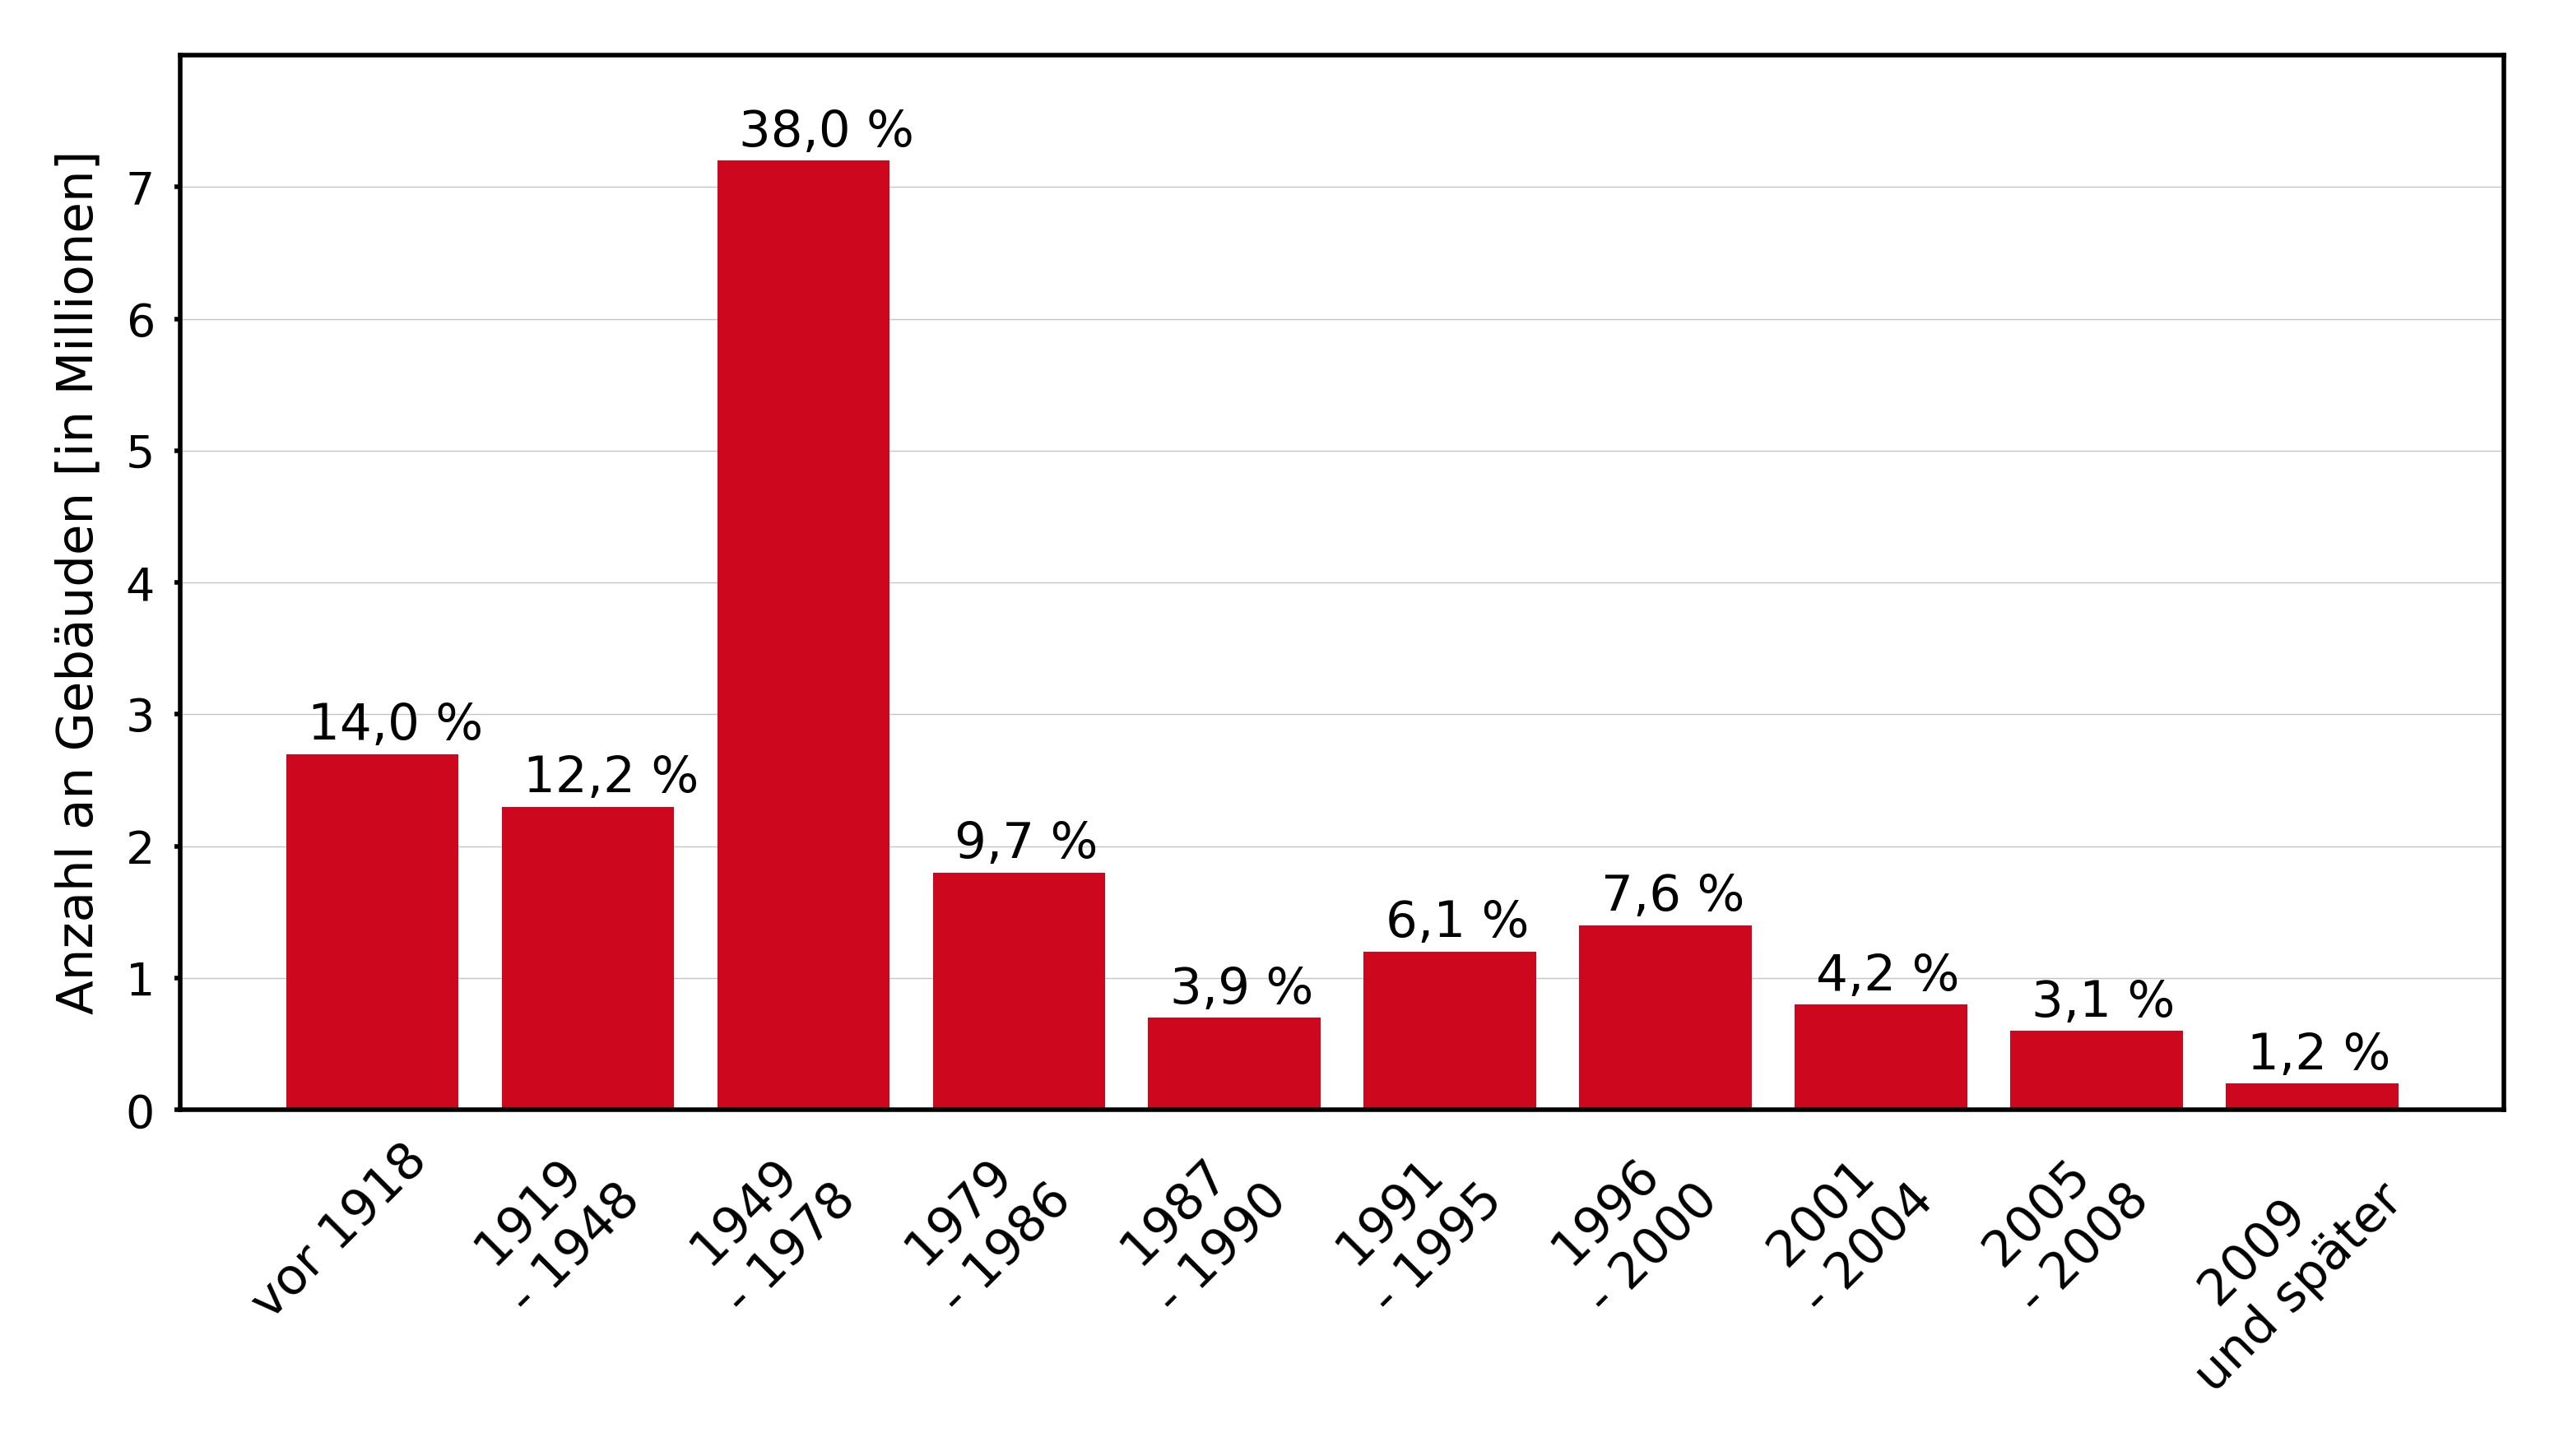
\includegraphics{Pictures/GebaeudeAlterDiagramm.jpg}
	\caption{errichtete Wohngebäude nach Mikrozensus-Klassen sowie deren Anteil am Gebäudebestand [in \%].\cite{StatistischeAmterdesBundesundderLander.2014}}
	\label{fig: Abbildung211} 
\end{figure}
%Zwanzig Jahre Klassen vorstellen?

Eine weitere Unterteilung des Wohngebäudebestandes erhält man bei der Betrachtung der Anzahl an Wohneinheiten im Gebäude. 
Hierbei setzt sich der Bestand zu zwei Dritteln aus Wohngebäuden mit nur einer Wohnung zusammen. 
Weitere \mbox{17 \%} bilden Gebäude mit zwei Wohnungen, während die Gebäudeklasse mit \mbox{3 - 6 Wohnungen} mit \mbox{12 \%} vertreten ist. 
Die größeren Gebäude mit \mbox{7 - 12 Wohnungen} sowie mit 13 und mehr Wohnungen sind anteilig am Gebäudebestand mit jeweils \mbox{5 \%} und \mbox{1 \%} relativ kleine Gruppen. 
Allerdings gelten letztere nur bei einer Gebäudebetrachtung als weniger relevant, da sie bei einer Anschauung der Wohneinheiten logischerweise mit größeren Faktoren im Vergleich zu Einfamilienhäusern einhergehen. \cite{StatistischeAmterdesBundesundderLander.2014b}
%einhergehen oder eingehen?

In Abbildung \ref{fig: Abbildung212} sind die Anzahl der Wohneinheiten für die drei Baualtersklassen älter als 1978, \mbox{1979 - 1994} und \mbox{1995 - 2009} sowie deren Anteil an allen Wohneinheiten bis Baujahr 2009 des Gebäudebestandes dargestellt. 
In Anlehnung an den vorherigen Abschnitt werden Gebäude mit bis zu 2 Wohnungen als Ein- und Zweifamilienhäuser zusammengefasst und nach der englischen Bezeichnung \glqq single family home\grqq\,mit SFH abgekürzt. 
Wohngebäude mit 3 oder mehr Wohnungen werden als Mehrfamilienhäuser mit der Abkürzung MFH für \glqq multy family home\grqq\,gebündelt. 

Auffallend ist wiederum der enorme Anteil der Gebäude mit Baualter älter als 1978. 
Hier zählen die Mehrfamilienhäusern mit 14,8 Millionen Wohnungen und einem Anteil aller bis 2009 errichteten Wohneinheiten von \mbox{38 \%} zur größten Gruppe. 
Mit 12,5 Millionen Wohnungen und einem Anteil von 32\,\% entfällt die zweitgrößte Klasse auf die Einfamilienhäuser mit Baujahr älter 1978.
Ähnlich wie zuvor bei der Gebäudebetrachtung wurden somit auch mehr als zwei Drittel aller Wohnungen vor 1978 erbaut.

\begin{figure}[H]
	\centering
		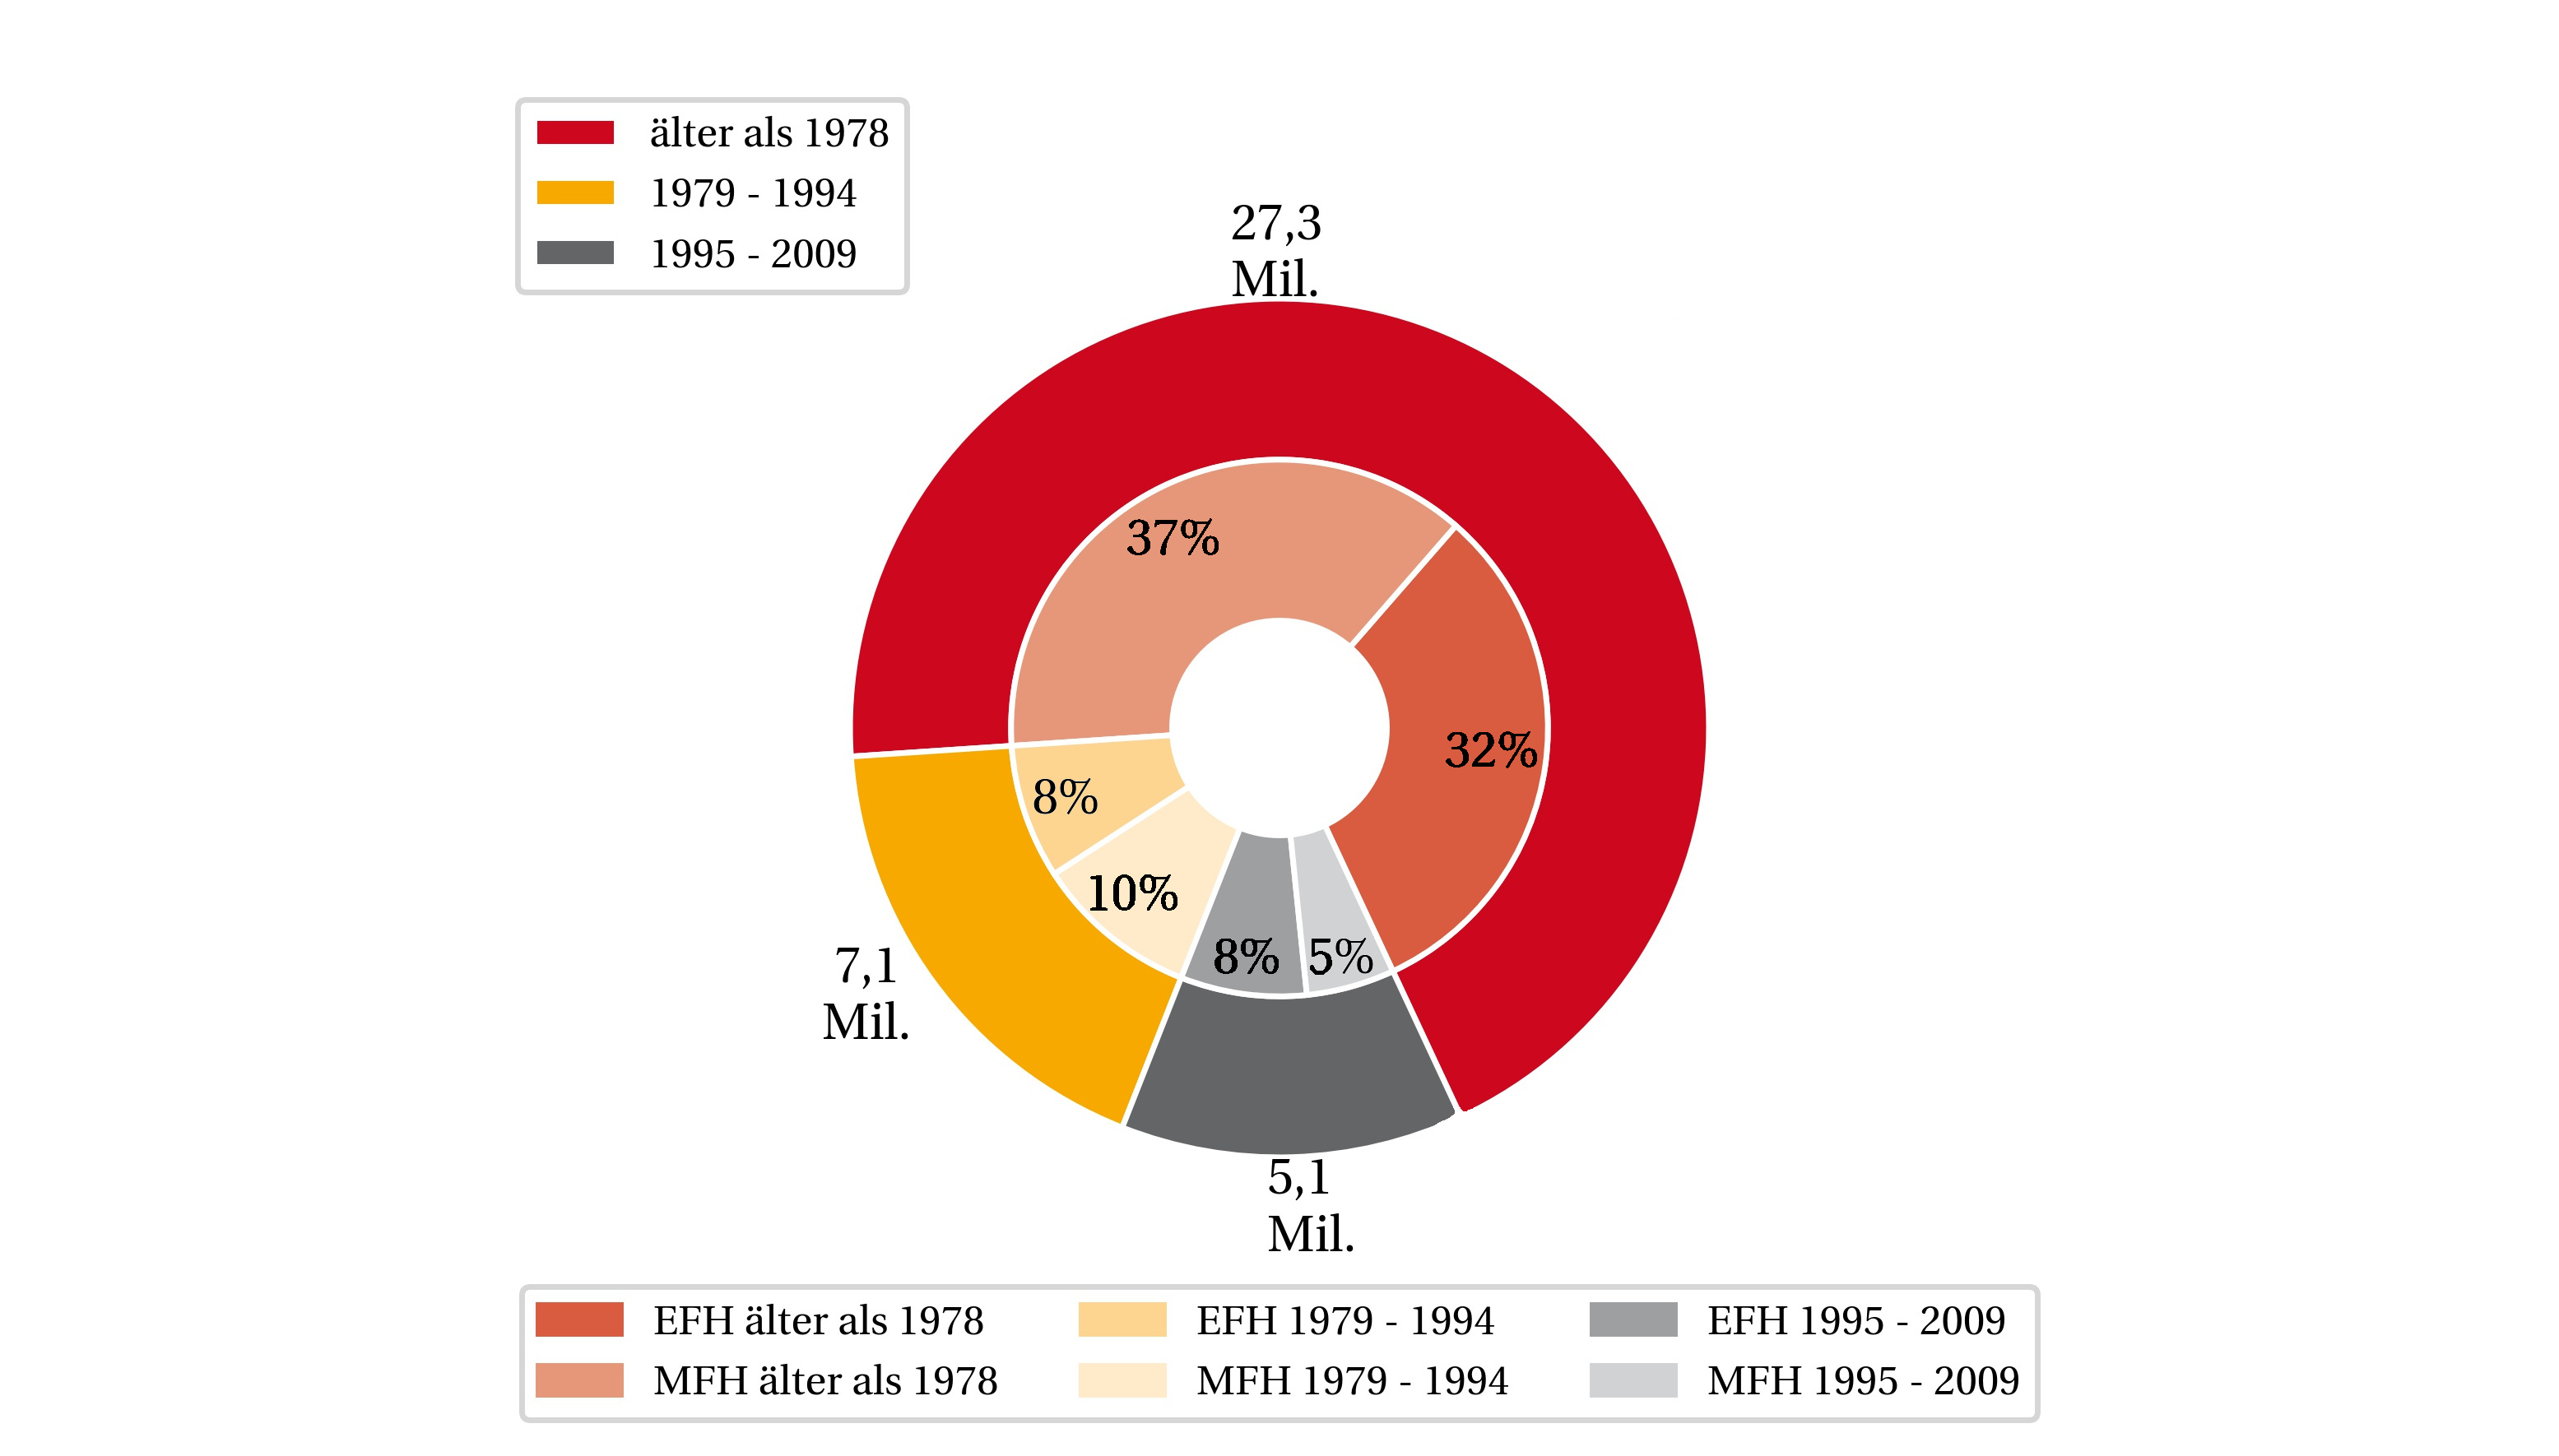
\includegraphics{Pictures/GebaeudeGroesse.jpg}
	\caption{Anzahl an Wohneinheiten bei Einfamilienhäuser (SFH) und Mehrfamilienhäuser (MFH) sowie deren relativer Anteil [in \%] nach Baualtersklassen. \cite{StatistischeAmterdesBundesundderLander.2014b}}
	\label{fig: Abbildung212} 
\end{figure}

Eine detailliertere Gliederung der Gebäudetypen ist in Tabelle \ref{tab: TabelleA0} zu finden. 
Hier wurden die Anzahl der Wohneinheiten nach Baualtersklasse und Gebäudetyp eingeteilt. 
Zu den zuvor beschriebenen Ein- und Mehrfamilienhäusern sind in der Tabelle außerdem die Klassen der Reihenhäusern (RH), großen Mehrfamilienhäuser (GMH) sowie Hochhäusern (HH) zu ermitteln. 
Weiter lassen sich die Anzahl der Wohnungen für diverse Gebäudearten in neuen Bundesländern (NBL) ablesen.

Zusammenfassend lassen sich folgende Punkte bei der statistischen Betrachtung des deutschen Gebäudebestandes festhalten:

\begin{itemize}
	\item $\nicefrac{2}{3}$ aller Gebäude und Wohnungen des Bestandes wurden vor der 1. Wärmeschutzverordnung 1978 errichtet.
	\item Bei einer Betrachtung der Wohneinheiten halbiert sich der Bestand in Gebäude mit einer oder zwei Wohnungen (47\,\%) und drei oder mehr Wohnungen (53\,\%).
	\item Gebäude, die nach der Jahrtausendwende gebaut wurden, bilden keinen großen Anteil des Bestandes.
\end{itemize}

%Wohnobjekte?
%Zensus näher erläutern?
%Typgebäude näher beschreiben?
%Auf Wohnfläche eingehen?
%Auf Unterschied zw neuen und alten Bundesländern eingehen?


\section{Historische Entwicklung der Gebäudehülle}
\label{sec:Sektion 22}

Nachdem im vorherigen Kapitel der Gebäudebestand nach Alter und Größe beschrieben wurde, werden nun die zu den jeweiligen Gebäudealtern zugehörigen Baustoffe und Dämmeigenschaften vorgestellt. 
Hierzu wird zwischen der Isolierung verschiedener Gebäudebauteilen unterschieden. 
Neben Möglichkeiten zur Dämmung des Daches beziehungsweise der obersten Geschossdecke und der Außenwand werden zudem die Dämmung des Bodens betrachtet.
Weiterhin wird auf den Verglasungsstandard verschiedener Epochen eingegangen.
%Warum Dach und oberste Geschossdecke zusammengefasst werden kurz erklären?

Ein wichtiger Kennwert zur energetischen Bewertung eines Gebäudes und einzelner Gebäudekomponenten beschreibt der U-Wert.
Hierbei handelt es sich um den Wärmeübergangskoeffizienten, welcher den Wärmestrom durch 1\,m² Bauteilfläche bei 1\,K Temperaturdifferenz beschreibt. 
Berechnet wird dieser als Kehrwert des Wärmedurchgangswiderstand \(R_T\). 
Der U-Wert ist definiert als
\begin{equation}
\label{eq:Gleichung221}
U = \frac{1}{R_T}  \ \ \ \ \ \ \ \text{in} \ \ W/(m^2 \cdot K)
\end{equation}
wobei mit
\begin{equation}
\label{eq:Gleichung222}
R_T = \sum \limits_{i} \frac{d_i}{\lambda_i}	
\end{equation}				%Muss ich da innere, äußere Schicht unterscheiden?
der Wärmedurchgangswiderstand als Verhältnis der Dämmstoffdicke \(d_i\) einer Dämmschicht \(i\) und der Wärmeleitfähigkeit \(\lambda_i\) des Baustoffes der Schicht \(i\) beschrieben wird. 

Für transparente Bauteile und somit explizit für Fenster variiert die Berechnung des Wärmedurchgangskoeffizienten \(U_w\):
\begin{equation}
\label{eq:Gleichung223}
U_w = \frac{A_g \cdot U_g + A_f \cdot U_f + l_g \cdot \psi_g}{A_g + A_f}  \ \ \ \ \ \ \ \text{in} \ \ W/(m^2 \cdot K)
\end{equation}
Hierbei beschreiben \(A_f\) den Flächenanteil des Fensterrahmens und \(A_g\) die Glasfläche. Ferner sind \(U_g\) und \(U_f\) die Wärmeübergangskoeffizienten der Verglasung (Index g) und des Fensterrahmens (Index f). 
Außerdem werden Wärmebrückenbildungen des Glasrandverbundes mit der Multiplikation des \(\psi\)-Wertes mit der Gesamtumfangsfläche der Verglasung \(l_g\) berücksichtigt. \cite{Laasch.2013}
%Wärmebrücken erklären?

Aus den Definitionen der U-Werte und des Wärmedurchgangswiderstandes lässt sich leicht erkennen, dass die Transmissionswärmeverluste eines Gebäudes stark von der Dicke und den Dämmeigenschaften des Dämmmaterials abhängen. 
Hierbei lassen sich historische Unterscheidungen treffen.

Die drei TABULA-Klassen \mbox{vor 1918}, \mbox{1919 - 1948} sowie \mbox{1949 - 1957} umfassen die Epochen der Gründerzeit, der Zwischenkriegszeit, den beiden Weltkriegen sowie der Nachkriegszeit. 
Wie in Kapitel \ref{sec:Sektion 21} bereits dargelegt, prägen die Nachkriegsjahre einen schnellen Wiederaufbau, in dem vor allem mit Trümmern neue Gebäude errichtet wurde. 
Auch in dem Zeitraum \mbox{vor 1918} kam es im Rahmen der Ausdehnung der Städte zu zahlreichen neuen Konstruktionen. 
Aus Tabelle \ref{tab: TabelleA1} lässt sich erkennen, dass sich die Wärmeübergangskoeffizienten der Gebäudetypen SFH und MFH in diesen Jahren stark ähneln. 
Dies ergibt sich auch aus der Darstellung der Geschichte des Dämmstandards von Eicke-Henning. %hier schon zitat?
Hier wurde festgehalten, dass sich bis zum Jahr 1957 die Dämmindustrie und der Hochbau im Rahmen der Industrialisierung zwar weiterentwickelte, es allerdings dennoch keinen Wandel im Hinblick auf Wärmeschutz gab.
So wurde bevorzugt günstig gebaut und die damit verbunden erhöhten Heizkosten in Kauf genommen.
Die im Jahr 1952 eingeführte DIN 4108 verkörperte zwar den ersten Ansatz Wärmeschutz normativ zu regulieren, jedoch konnte sie auch zu keiner Veränderung der energetischen Bauweise führen. 
Trotz deren Name \glqq Wärmeschutz im Hochbau\grqq\,beinhaltete die Norm nur einen Mindestwärmeschutz zur Vermeidung bauphysikalischer Schäden durch Schimmelbildung.
Als Standard dieser Jahre galt das 38\,cm dicke Vollziegel-Mauerwerk, Böden und Dächer ohne Dämmung sowie die Einscheiben-Verglasung. \cite{EickeHenning.2011}

In den folgenden Jahren von \mbox{1958 - 1968} sowie \mbox{1969 - 1978} kam es zu keinen normativen Änderungen des Wärmeschutzes. 
Dennoch kann durch einen Wandel der Baustoffwahl eine Verbesserung der U-Werte beobachtet werden. 
So verschwand der Vollziegel langsam vom Markt und wurde durch Hochlochziegeln oder Hohlblocksteinen substituiert.
Weiter wurden vermehrt Trittschalldämmungen in Böden und Dächer installiert. 
Trotz deren primären Zweckes der Lärmvermeidung erzielten diese dünnen Dämmschichten von \mbox{1 - 4 cm} eine Verbesserung der Wärmedurchgangskoeffizienten der zuvor genannten Bauteile.
Ab 1965 erreichten vorgefertigte Betonteile mit einem \mbox{3 - 6 cm} dicken Dämmkern zudem einen besseren Wärmeschutz.
Bezüglich der Fenster wurde in diesen Jahren keine Veränderung geschaffen, so dass weiterhin die Einscheiben-Verglasung die Konvention bildete. \cite{EickeHenning.2011}

Nach der Ölkrise von 1974 rückte die Bedeutung des ressourcenschonenden Bauens beziehungsweise Betriebes von Gebäuden in den Vordergrund. 
Der Gesetzgeber verabschiedete am 11. August 1977 mit der 1. Wärmeschutzverordnung, im Folgenden mit WschV abgekürzt, erstmalig eine Verordnung, in der ein Standard zur Minimierung des Heizwärmebedarfs festgelegt wurde. 
In Folge der 1. WschV verbesserte sich die Dämmeigenschaften der Bauten mit Baujahr \mbox{1979 - 1983}.
So lässt sich bei den TABULA SFH-Typgebäude dieser Jahrgänge feststellen, dass sowohl das Dach eine 8\,cm als auch der Boden eine 4\,cm dicke Dämmschicht besitzen. 
Dadurch konnten U-Werte von 0,5\,\(W/(m^2 \cdot K) \) für das Dach sowie 0,65\,\(W/(m^2 \cdot K) \) für den Boden erreicht werden (s. Tabelle \ref{tab: TabelleA1}).
Weiterhin wurde durch die Verordnung vorgeschrieben, dass \glqq außenliegende Fenster und Fenstertüren von beheizten Räumen (...) mindestens mit Isolier- und Doppelverglasung auszuführen (sind)\grqq \cite{Bundesregierung.1977}.
Somit ermöglichte die 1. WschV eine Verbesserung des energetischen Standards der Wohngebäuden. 
Allerdings stellten die ersten normativen Anforderungen an die Gebäudehülle aus heutiger Sicht nur einen Zwischenschritt hin zu einem energetisch sinnvollen Reglement dar.
Als Beispiel hierfür ist die Anforderung an Fenster zu nennen. 
Für diese wurde in der 1. WschV festgelegt, dass ein U-Wert von 3,5\,\(W/(m^2 \cdot  K) \) nicht überschritten werden darf \cite{Bundesregierung.1977}.
Nach heutigem Standard der Energieeinsparverordnung 2009, die im Folgenden noch weiter erläutert wird, sind für die Fenster im Neubau \(U_w\)-Werte kleiner 1,3\,\(W/(m^2 \cdot K) \) einzuhalten.
Bei diesem Vergleich ist auch noch festzuhalten, dass es sich bei der Vorgabe zum U-Wert der 1. WschV um den \(U_g\)-Wert handelt, der nur den Wärmedurchgang durch die Verglasung beschreibt und somit im Gegensatz zu \(U_w\) weder den Wärmeübergang durch den Rahmen noch die Wärmebrückenbildung beachtet. 
Daher liegt der von TABULA ermittelte \(U_w\)-Wert für das SFH-Typgebäudenfenster der Jahre \mbox{1979 - 1983} aufgrund dessen energetisch schlechten Metallrahmen mit 4,3\,\(W/(m^2 \cdot K) \) höher als der \(U_g\)-Normwert der 1. WschV. \cite{EickeHenning.2011} 
%Bsp mit EnEV ok? Zeitstrahl wäre nice

Einen weiteren Schritt hin zu einem besseren Wärmeschutz des Gebäudebestandes markiert die 1982 beschlossene und 1984 in Kraft getretene 2. WschV, die sich auf den Wärmeschutz der Gebäude mit Baujahr \mbox{1984 - 1994} auswirkte.
Nach Eicke-Henning kann sich \glqq das Niveau von 1984 (...) mit 2-Scheiben-Isolierverglasung, 30\,cm dicken porosierten Außenwänden (...), 8-9\,cm Wärmedämmung im Dach und 4\,cm Kellerdämmung beschreiben (lassen) \grqq\,\cite{EickeHenning.2011}.
Wie sich aus Tabelle \ref{tab: TabelleA1} lesen lässt, führten die Maßnahmen der 2.\,WschV zu einem durchgehend besseren Verhalten der Bauteile gegenüber Transmissionswärmeverluste. 
Im Bezug auf die Anforderung der Fensterflächen ergab sich zwar eine Verbesserung im Vergleich zur 1.\,WschV auf \(U_{g, max} = 3,1\,W/(m^2 \cdot K) \), allerdings blieb die im vorangegangenen Abschnitt diskutierte Problematik des \(U_g\)-Wertes erhalten.
Des Weiteren definierte die 2. WschV Anforderungen an \glqq Bauliche Änderungen bestehender Gebäude\grqq.
Daraus folgte, dass bei Gebäudeerweiterungen oder Umbaumaßnahmen das betroffene Bauteil den geforderten energetischen Neubaustandard erfüllen musste.

Einen Paradigmenwechsel des Wärmeschutzes kennzeichnete die 3.\,Verordnung über einen energiesparenden Wärmeschutz bei Gebäuden von 1995.
Im Gegensatz zu den zuvor vorgestellten Verordnungen begrenzte die 3.\,WschV nicht nur die U-Werte der Bestandteile der Gebäudehülle, sondern beschränkte zudem den Jahres-Heizwärmebedarf.
Als Folge der neuen Verordnung erhielten die Bauteile im Vergleich zur 2. WschV \mbox{4 - 6 cm} mehr Dämmdicke. 
Außerdem wurde durch die erhöhten Anforderungen an die Verglasung die Zweischeiben-Wärmeschutzverglasung der Neubaustandard.
Aufgrund dieser Maßnahmen konnten die U-Werte der Gebäude mit Baujahr \mbox{1995 - 2001} signifikant gesenkt werden.
Besonders die bessere Verglasung mit wärmetechnisch besseren Rahmen erzielte eine Verbesserung des \(U_g\)-Wertes von \mbox{3 - 3,2 \(W/(m^2 \cdot K) \)} auf 1,9\,\(W/(m^2 \cdot K) \).

Die zum 01. Februar 2002 in Kraft getretene Energieeinsparverordnung (EnEV) legte die zuvor genannte 3. WschV sowie die Heizungsanlagenverordnung zusammen. 
Somit wurden alle Anforderungen an den Energieverbrauch eines Gebäudes in einer Verordnung gebündelt.
Anstelle der Begrenzung des Jahres-Heizwärmebedarfes, wie im Abschnitt zuvor, wurde der Jahres-Primärenergiebedarf sowie der flächenspezifische Transmissionswärmeverlust (\(H_t'\)) limitiert.
Obwohl nicht explizit strengere Regulationen an die Gebäudehülle formuliert wurden, konnte durch die Restriktion von \(H_t'\) ein Absinken der Wärmedurchgangskoeffizienten aufgrund dickerer Dämmschichten erzielt werden.
Nach Tabelle \ref{tab: TabelleA1} sank der U-Wert des Zeitraumes \mbox{2002 - 2009} für alle Komponenten der Gebäudehülle im Rahmen der \mbox{EnEV 2002}.
Außerdem setzte die Verordnung striktere Anforderungen an den Altbaubestand. 
So mussten vor dem 01.10.1978 eingebaute Heizkessel mit flüssigem oder gasförmigen Brennstoff ersetzt werden, ungedämmte und zugängliche Wärmeverteilungs- und Warmwasserleitungen nachgedämmt werden sowie nicht begehbar, zugängliche oberste Geschossdecken auf einen U-Wert von 0,3 \(W/(m^2 \cdot K) \) gedämmt werden.
%Energieausweis

Auf die EnEV 2002 folgten 2004 sowie 2007 Novellierungen.
Diese stellten keine Verschärfung der energetischen Anforderungen nach EnEV 2002 dar, sondern galten der Beseitigung juristischer Problematiken sowie der Einführung des Energieausweises für Bestandsgebäude \cite{Wild.2015}.
Eine solche Verschärfung wurde durch die EnEV 2009 vollzogen.
Zum einen wurde die Berechnung des Jahres-Primärenergiebedarfes umgestaltet.
Das Berechnungsverfahren nach EnEV 2009 bestimmte einen flächenspezifischen Höchstwert des Jahres-Primärenergiebedarfes, welcher durch ein Referenzgebäude gleicher Geometrie, Gebäudenutzfläche und Ausrichtung kalkuliert wurde.
Die U-Werte der Referenzgebäudeberechnung wurden von TABULA für die Typgebäude der Baujahre \mbox{2010 - 2015} übernommen und sind in Tabelle \ref{tab: TabelleA1} zu finden.
Zum anderen wurden die Grenzwerte \(H_{t, max}'\) in weniger Kategorien als EnEV 2002 unterteilt und verschärft.
%EnEV Zitate

\begin{figure}[H]
	\centering
		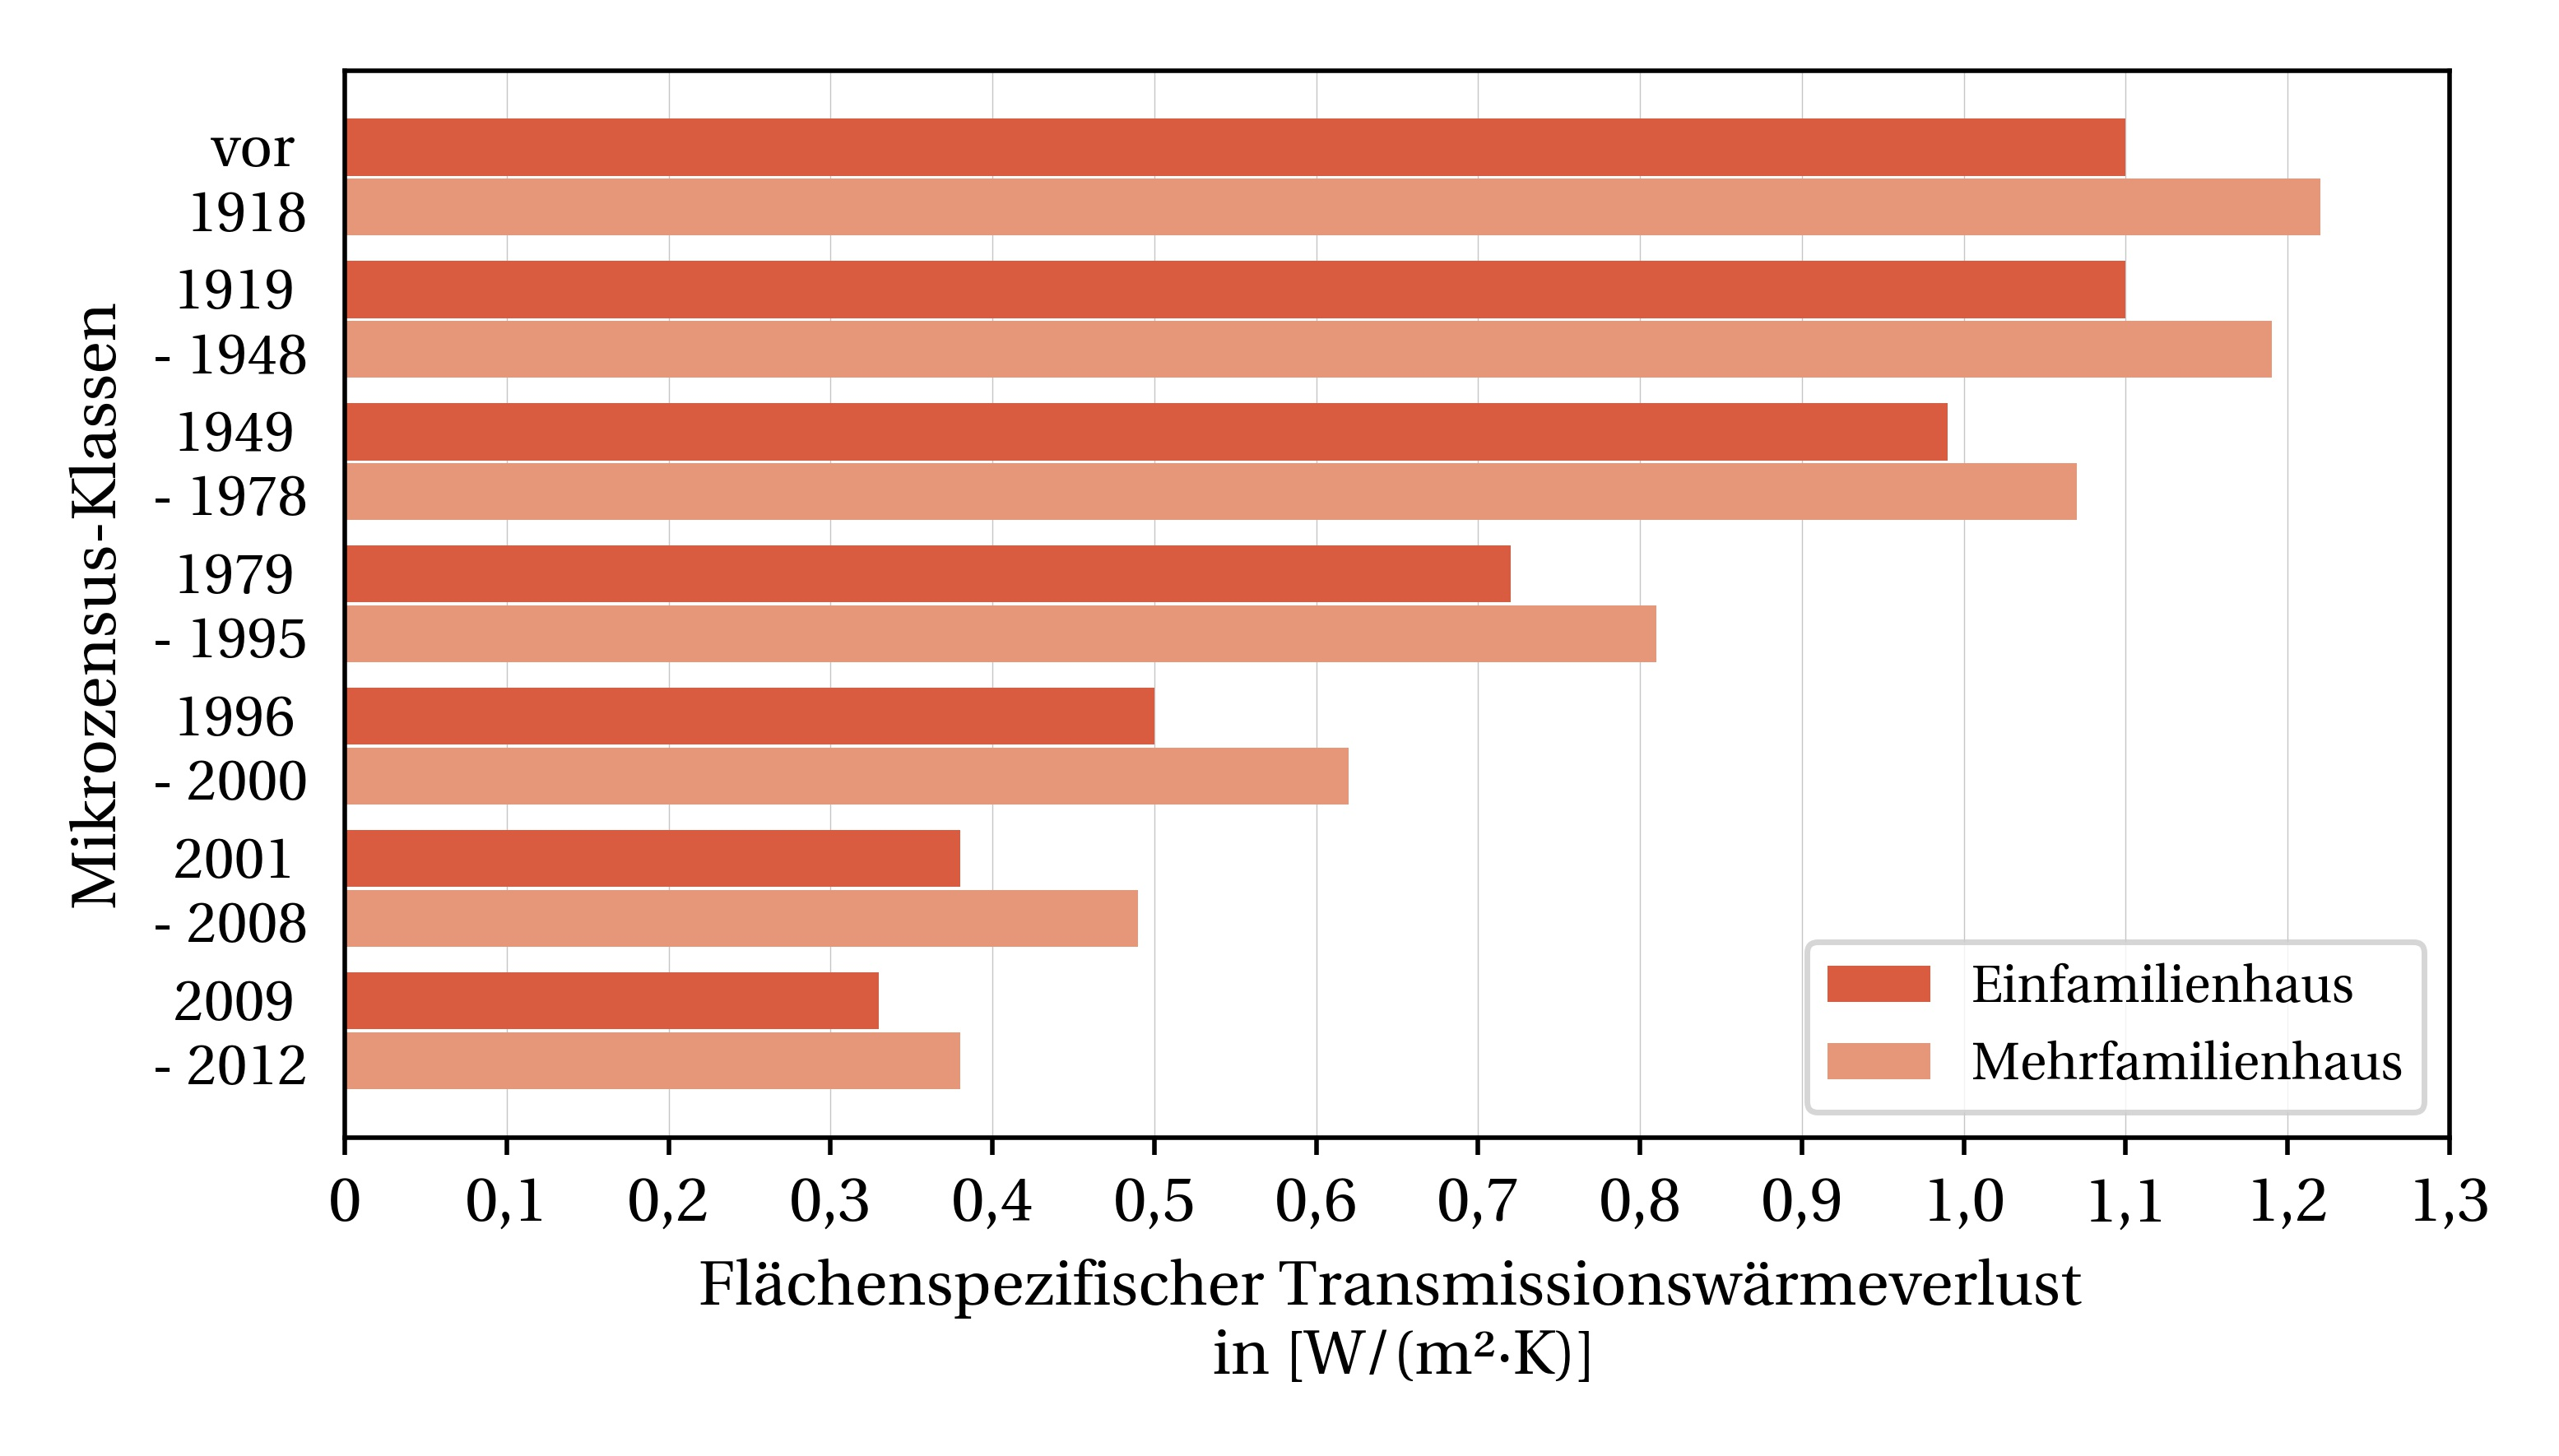
\includegraphics{Pictures/TransmissionswaermekoeffizientBaujahr.jpg}
	\caption{Flächenspezifischer Transmissionswärmeverlust \(H'_t\) nach Baujahr und Gebäudeart. \cite{Bigalke.2016}}
	\label{fig: Abbildung221} 
\end{figure}

Abbildung \ref{fig: Abbildung221} zeigt den flächenspezifischen Transmissionswärmeverlust der Gebäudetypen SFH sowie MFH für verschiedene Baujahre. 
Zu erkennen ist zum Einen, dass die Werte der MFH immer über denen der SFH liegen und zum Anderen die kontinuierliche Verbesserung im Zuge der energetisch günstigeren Gestaltung der Wohngebäude.
Weiterhin ist festzustellen, dass durch die Wärmeschutz- und Energieeinsparverordnungen der letzten 40 Jahre die flächenspezifische Transmissionswärmeverluste der Neubauten um Vergleich zu einem Altbau um fast 75\,\% gesunken sind.

Zu Tabelle \ref{tab: TabelleA1} ist anzumerken, dass sie sich auf den Zustand der Bauteile im damaligen Neubau bezieht. 
Einzige Ausnahme hierbei bilden die Fenster der Zeiträume bis 1978. 
Für diese charakterisiert die Einscheiben-Verglasung den Einbau-Zustand, allerdings wurde im Rahmen diverser Förderprogramme der Großteil der Einscheiben-Verglasungen durch Zweiglas-Fenster ersetzt.
%Hier doof
%Zeitstrahl mit Transmissionswärmeverlusten
%Auf Grafik Bezug nehmen


\section{Sanierungsstand des deutschen Wohngebäudebestandes}
\label{sec:Sektion 23}

In dem vorangegangen Abschnitt wurde die Entwicklung der Gebäudehülle vorgestellt. 
Hierbei wurde sich auf den Neubauzustand bei Fertigstellung des Gebäudes bezogen.
Dieses Kapitel soll nun die Veränderung des Gebäudebestandes durch energetische Sanierung veranschaulichen.

Abbildung \ref{fig: Abbildung231} zeigt den Anteil der durch nachträgliche Wärmedämmung sanierten Bauteilflächen nach Bauteilen und Gebäudeart.
Zu erkennen ist der große Anteil an sanierter Dachfläche beziehungsweise obere Geschossdeckenfläche.
Dieser liegt für SFH und MFH annähernd gleich bei etwa 57\,\%.
Folglich wurden mehr als die Hälfte der Dachflächen im Altbau nachträglich gedämmt.
Einen leichten Unterschied zwischen den Gebäudearten ist bei den nachträglich sanierten Außenwänden zu beobachten. 
Bei diesem Bauteil wurden bei MFH etwas mehr als 31\,\% mit einer besseren Dämmung versehen, wohingegen es bei den SFH nur etwa ein Viertel waren.
Deutlich weniger Relevanz bei der nachträglichen Dämmung erhielt die Isolierung des Fußbodens beziehungsweise der Kellerdecke. 
Für diese Bauteile wurden bei beiden Gebäudearten nur circa 10\,\% mit einem besseren Wärmeschutz versehen. 

In Abbildung \ref{fig: Abbildung231} fehlen die Angaben zum Sanierungsstand der Fenster.
Hierfür ist die Datenlage der Sanierung schwierig, allerdings bietet das IWU eine Schätzung über den Bestand an Fenstern im Jahre 2015 \cite{Bigalke.2016}.
Tabelle \ref{tab: TabelleA2} gibt verschiedene Verglasungsarten mit deren \(U_g\)-Werten sowie Anzahl und Anteil am gesamten Fensterbestand in Deutschland wieder.
Wie in Gleichung \ref{eq:Gleichung223} dargelegt, beschreibt der \(U_g\)-Wert den Wärmedurchgang durch die Verglasung ohne Berücksichtigung des Fensterrahmens oder der Wärmebrückenbildung.

Obwohl die Einfachverglasung für einen großen Teil des Altbaues den Neubaustandard darstellte, ist deren Anteil am Fensterbestand mit nur noch 3\,\% sehr gering. 
%Aufgrund dessen enorm hohen Wärmedurchgangskoeffizient in Höhe von 5,8\,\(W/(m^2 \cdot K)\) ist die Rückläufigkeit dieser Fensterart als positiv zu bewerten.
Der heutige Bestand der Fenster wird durch unbeschichtetes Isolierglas sowie dem Zweischeiben-Wärmedämmglas dominiert, welche mit 34\,\% und 47\,\% vertreten sind.
Weiterhin ist zu erkennen, dass das Dreischeiben-Wärmeglas bereits 8\,\% des Fensterbestandes stellt, obwohl dieses erst 10 Jahren vor Erhebung der Daten auf den Markt kam.

\begin{figure}[H]
	\centering
		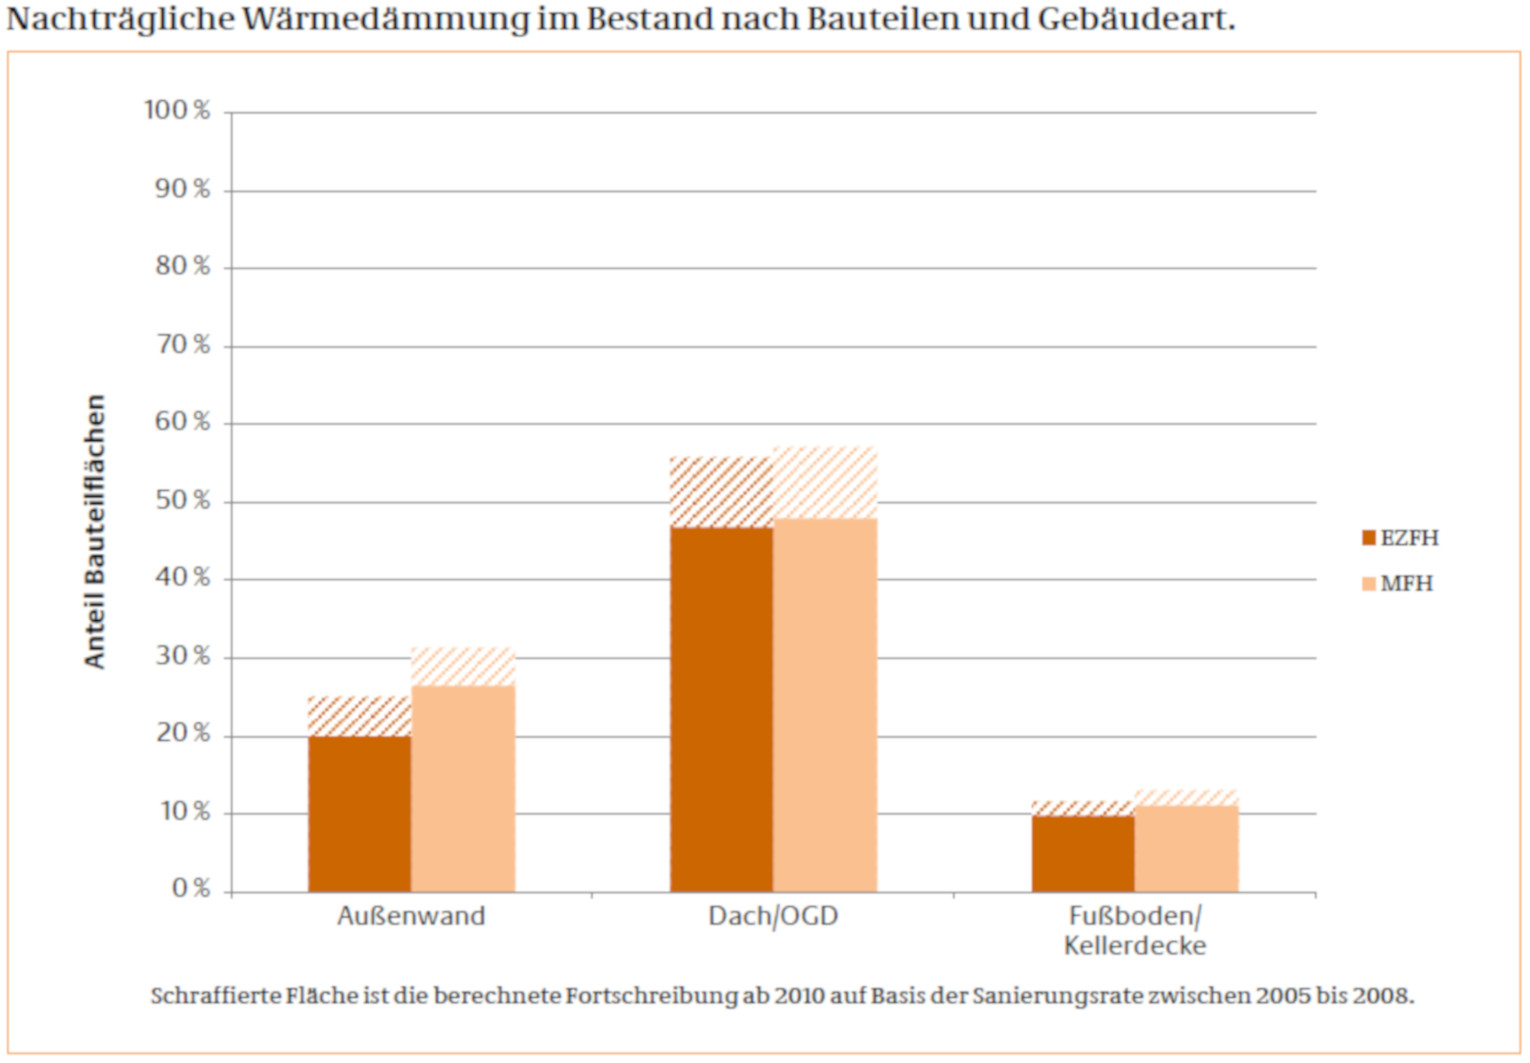
\includegraphics{Pictures/NachtraeglicheSanierung.jpg}
	\caption{Anteil der Gebäudetypen Ein- und Zweifamilienhäuser sowie Mehrfamilienhäuser mit nachträglicher Dämmung der Bauteile Außenwand, Dach/Obergeschossdecke und Fußboden/Kellerdecke \cite{Bigalke.2016}}
	\label{fig: Abbildung231} 
\end{figure}


\section{Förderprogramme}
\label{sec:Sektion 24}

In Kapitel \ref{sec:Sektion 22} werden diverse Verordnungen zum besseren Wärmeschutz des deutschen Gebäudebestandes beschrieben.
Diese verkörpern Anforderungen an den Neubau oder an Einzelsanierungsmaßnahmen und nur wenige Forderungen an den Bestand.
Zur Steigerung der Wirtschaftlichkeit solcher Sanierungsmaßnahmen unterstützt die Bundesrepublik Gebäudeeigentümer finanziell bei energetischen Sanierungsvorhaben.

Als Beispiel eines erfolgreichen Förderprogrammes sei der Rückgang der Einfachverglasung genannt.
Im Rahmen des Energiespar-Förderprogrammes investierte die Bundesregierung ab 1977 4,35 Milliarden DM zur Erneuerung von Heizungen und Fenster \cite{EickeHenning.2011b}.
Dadurch konnte ein Anreiz zur energetischen Sanierung geschaffen werden, was mit einen Grund darstellt, dass der Anteil an Einfachverglasung heute nur noch etwa 3\,\% beträgt.


%Aktuelle Förderprogramme ergänzen


\section{Arten der Optimierung}
\label{sec:Sektion 25}

Ziel dieser Arbeit ist die Bestimmung verschiedener Maßnahmen, welche für repräsentative Gebäudetypen eine wirtschaftlich und ökologisch optimale Lösung bieten.
Hierbei werden neben verschiedenen Möglichkeiten der Energiebereitstellung auch die Qualität und Verbesserung verschiedener Komponenten der Gebäudehülle betrachtet.
Dadurch ergibt sich eine enorm hohe Anzahl an möglichen Kombinationsmöglichkeiten der Maßnahmen.
Um aus dieser Komplexität ein Optimum zu bestimmen, ist es unabdingbar ein rechnergestütztes Optimierungsprogramm als Werkzeug zu benutzen.

In einem mathematischen Sinne beschreibt die Optimierung die Lösung einer Zielfunktion.
Diese Funktion wird mit Variablen beschrieben und mit Rahmenbedingungen, Restriktionen genannt, beschränkt \cite{Schellong.2016}.
Somit wird mit einem Optimierungsprogramm versucht, eine Problematik mathematisch zu modellieren, um eine rationale Entscheidung über eine optimale Lösung zu treffen. 
Im Folgenden stellt dieses Kapitel verschiedene Arten der Optimierung sowie diverse Optimierungsprogramme vor, um letztlich das im Rahmen dieser Arbeit verwendete Programm in \ref{sec:Sektion 26} beschreiben zu können.

Zur Einteilung von Optimierungsprogrammen existieren verschiedene Möglichkeiten.
Bei der Betrachtung der zu Grunde liegenden Variablen erhält man eine Unterteilung.
Hierbei werden die Programme in einem mathematischen Sinne danach unterteilt, aus welchem Raum die Variablen entstammen.
So wird zwischen diskreten und kontinuierlichen Variablen unterschieden. 
Die diskreten entstammen aus \(\mathbb{Z	}\) und umfassen unter anderem ganze Zahlen und Binärvariablen.
Letztere sind die Menge aus [0; 1] und werden im Rahmen der Optimierung oft als Option der Kaufentscheidung oder Schaltzustände genutzt. %Kursiv?
Dabei beschreibt 0 einen ausgeschalteten, beziehungsweise nicht gekauften Zustand und 1 den eingeschalteten/gekauften.
Neben den diskreten Variablen werden auch kontinuierliche in Optimierungsprogrammen genutzt. 
Diese sind als reelle Zahlen \(\mathbb{R}\) definiert und beschreiben beispielsweise Kapazitäten, Heizbedarf oder Wärmeverluste.
Werden in einem Programm diskrete und kontinuierliche Variablen gemischt, so spricht man von einer gemischt-ganzzahligen Optimierung. \cite{Schellong.2016}

Neben den Variablen stellt die Art der Funktionen eine weitere Unterscheidung der Optimierungsprogramme dar.
Bestehen die Restriktionen und die Zielfunktion eines Programmes einzig und alleine aus linearen Zusammenhängen, so wird von einem linearen Programm (LP) gesprochen.
Dem Gegenüber werden solche Optimierungen, die auch Nichtlinearitäten abbilden, als nicht-lineare Programme (NLP) bezeichnet.
Oftmals findet man in der Realität nicht-lineare Zusammenhänge, welche mit NLP gut modelliert werden können.
Als ein Beispiel sei hier das Teillastverhalten von Wärmeerzeugern genannt.
Jedoch stellt das Lösen von nicht-linearen Gleichungen einen erhöhten Rechenaufwand dar, welcher mit einer deutlich längeren Rechendauer einhergeht.
Somit kann durch die Linearisierung von nicht-linearen Zusammenhängen Rechenzeit zu Kosten von Genauigkeitsverlusten verkürzt werden. 
Die gemischt-ganzzahlige lineare Optimierung wird aufgrund ihrer englischen Bezeichnung (\glqq Mixed Integer Linear Programing\grqq)\,mit MILP abgekürzt sowie die nicht-lineare analog mit MINLP. \cite{Samsatli.2018} %Anführungszeichen?

In der Literatur werden verschiedene Ansätze und Modelle für Optimierungen von Energiesystemen verfolgt, welche im Weiteren kurz vorgestellt werden.

Iturriaga et al. \cite{Iturriaga.2017} erarbeiten ein allgemeines Modell für Gebäudeenergiesysteme auf Gebäudeebene. 
Dieses soll alle derzeit verfügbaren Technologien der Wärme-, Kälte- und Elektrizitätsbereitstellung abbilden können.
Hierzu werden die Anlagen unterteilt in solche, die hohe, mittlere und niedrige Temperaturen erzeugen, sowie Kältemaschinen und elektrische Module.
Thermische und elektrische Energie kann zwischen den jeweiligen Gruppen ausgetauscht werden, um letztlich den Wärme-, Kälte- und Elektrizitätsbedarf des Gebäudes zu decken.
Weiterhin berücksichtigt das Modell neben der Energieerzeugung auch Speicher und Interaktionen mit anderen Gebäuden durch Nah-, Fernwärme- sowie Stromnetzen.
Die stückweise Linearisierung des nicht-linearen Teillastverhaltens der Anlagen führt zu rein linearen Gleichungen und somit einem MILP Problem.
Als Zielfunktion ist die Minimierung der annualisierten Kosten definiert. 
Diese setzen sich aus Investitionskosten, jährlichen variablen Kosten, Energiebezugskosten sowie Gewinnen aus dem Verkauf an überschüssiger Wärme, Kälte oder Elektrizität zusammen.
Als Restriktionen der Optimierung sind technologische Nebenbedingungen der oben genannten Gruppen, die Bedarfserfüllung des Energiesystems, gebäudespezifische Rahmenbedingungen sowie Begrenzungen der Variablen aufgeführt.
Zuletzt wird das Modell anhand eines Beispielgebäudes im nordspanischen Bilbao getestet.
Hierbei werden 13 verschiedenen Technologien der Wärme- und Elektrizitätserzeugung in Betracht gezogen.
Diese umfassen neben Organic-Rankine-, Gasturbinen- und Verbrennungsmotoren-Blockheizkraftwerke (BHKW) auch verschiedene solarthermische Anlagen (CPC, Vakuumröhrenkollektoren, Flachkollektoren), Biomasse-, Gas- und Brennwertkessel, Luft-Wasser-Wärmepumpen und diverse Photovoltaik-Anlagen (amorphe, mono- und polykristalline Solarmodule).

In \cite{Pinzon.23.04.201726.04.2017} wird von Pinzon et al. ein Modell zur Optimierung der Stromkosten unter Berücksichtigung der Behaglichkeit der Bewohner vorgestellt.
Hierbei werden neben Stromkosten aus Heiz- oder Kühlzwecken, Beleuchtung und Ersparnissen aus Photovoltaik (PV) und Energiespeichern auch thermische Lasten in den modellierten Zonen betrachtet.
Wie in Iturriaga et al. \cite{Iturriaga.2017} wird zunächst ein MINLP Modell erstellt, dass daraufhin durch stückweise Linearisierung in ein MILP gewandelt wird.
Als Zielfunktion ist die Minimierung des Strombedarfes und somit der Stromkosten beschrieben.
Der Bedarf setzt sich aus dem Verbrauch der zuvor genannten Komponenten zusammen.
Als Nebenbedingungen werden die Nutzung der PV-Anlagen und Energiespeicher, des Klimageräts und der Beleuchtung sowie der Einhaltung des thermischen Komforts definiert.
Bei Letzterem werden auch die Wärmeträgheit des Luftvolumens im Raum, sowie der Wärmeverlust durch den Infiltrationsluftvolumenstrom, also durch Undichtheiten in der Gebäudehülle, berücksichtigt.

In Risbeck et al. \cite{Risbeck.2017} wird der optimale Betrieb von Lüftungssystemen zum Kühlen und Wärmen in kommerziellen Gebäuden, also Nichtwohngebäuden, untersucht.
Hierzu werden diskrete Variablen zum Modellieren des An- und Abschaltens der Komponenten sowie kontinuierliche zur Abbildung der Lasten und Speicherstände genutzt.
Als Zielfunktion werden minimale Betriebskosten bei Einhaltung des thermischen Komforts im Gebäude formuliert.
Auch Risbeck et al. wandeln nicht-lineare Geräteverhalten durch stückweise Linearisierung in lineare um.
Dadurch wird die Rechenzeit verkürzt und das Programm kann in Echtzeit auf Preisänderungen, Bedarfsschwankungen und Wetteränderungen eingehen.
Als Nebenbedingungen der Optimierungsaufgabe wird neben der Temperierung verschiedener Gebäudezonen auch die optimale Nutzung der zur Verfügung stehenden Speicher beachtet.

Zhu et al. \cite{Zhu.2019} beschäftigen sich mit der Kapazitätsauslegung thermischer und elektrischer Speicher in Gebäudeenergiesystemen mit mehreren Energiebereitstellungsformen. 
Der Bedarf an elektrische Energie wird hierbei entweder durch Photovoltaik (PV), Netzbezug oder einer Batterie gedeckt. 
Zur Erfüllung des Wärmebedarfs stehen neben einer Wärmepumpenheizung noch ein sensibler Wasserspeicher zur Verfügung.
Ein Teil der nicht-linearen Gleichungen werden linearisiert. Da jedoch noch nicht-lineare Zusammenhänge in dem Programm existieren, handelt es sich bei dem Modell um ein MINLP.

Eine Betrachtung der Gebäudehülle ist in Asadi et al. zu finden \cite{Asadi.2012}.
Hierbei handelt es sich zum einen um ein MINLP und zum anderen um eine Parteo-Optimierung, bei welcher dem Programm mehrere Zielfunktionen übergeben werden.
Das Modell betrachtet neben Dämmarten und -dicken der Außenwand und des Dachs auch den Fenstertyp sowie Solarkollektoren. 
Hierzu wird für jedes Bauteil zwischen unterschiedlichen Sanierungsmaßnahmen unterschieden, allerdings wird das Programm auf die Wahl eines Szenarios je Bauteil eingeschränkt.
Weiter wird der Energiebedarf des Gebäudes vereinfacht als Summe des Wärme-, Kälte- und Warmwasserbedarfes berechnet.
Ziel des Programmes ist die Bestimmung des kosten- und emissionsoptimalen Energiesystem.

In \cite{Wouters.2014} modellieren Wouters et al. Haushalte, die auf Quartiersebene thermische und elektrische Energie untereinander austauschen können.
An Anlagentechnik stehen Brennwertkessel, BHKWs , thermische und elektrische Speicher, PV-Anlagen und kleine Windkraftanlagen (WKA) zur Verfügung.
Als Zielfunktion ist die Minimierung der Annuität durch optimale Anlagenwahl, -auslegung und -betrieb definiert.
Das Programm wird nur mit linearen Gleichungen modelliert, sodass es sich um ein MILP handelt.
Weiter werden Einflüsse regulatorischer Maßnahmen untersucht und darauf aufbauend zwei Standorte mit ähnlichen klimatischen Bedingungen in Griechenland und Australien miteinander verglichen.

Das Optimierungsmodell von Harb et al. \cite{Harb.2016} bestimmt die optimale Anlagenauswahl zur Wärmeerzeugung von Einzelwohngebäuden oder Quartieren.
Es werden Mikro-BHKWs, Wärmepumpen, Elektroheizstäbe, PV, thermische Speicher, Kessel sowie Nahwärmenetze in Betracht gezogen.
Besonders an dem Modell von Harb et al. ist weiterhin, dass die Einspeisevergütung von PV-Strom sowie die Förderung von BHKW produzierter Elektrizität in die wirtschaftliche Betrachtung mit eingehen.

\section{Referenzmodell}
\label{sec:Sektion 26}

Als Grundlage dieser Arbeit liegt ein Programm zur Kosten- oder Emissionsoptimierung von Gebäudeenergiesystemen vor.
Neben einer Auswahl an Anlagentechnik zur Energiebereitstellung stehen außerdem Sanierungsmaßnahmen der Gebäudehülle zur Verfügung. 
Hierbei wird ähnlich wie bei Asadi et al. \cite{Asadi.2012} Außenwände, Fenster und Dächer sowie zusätzlich Böden betrachtet.
Die Entscheidung für verschiedene Anlagen oder Maßnahmen an der Hülle erfolgt durch diskrete Binärvariablen, wohingegen die Auslegung und der Betrieb durch kontinuierliche Variablen modelliert wird.
Wie in Iturriaga et al. \cite{Iturriaga.2017}, Pinzon et al. \cite{Pinzon.23.04.201726.04.2017} und Risbeck et al. \cite{Risbeck.2017} erfolgt eine Linearisierung der nicht-linearen Gleichungen, sodass es sich um ein MILP handelt.
Die Zielfunktion der Optimierung kann entweder zur Minimierung der Kosten oder CO\(_2\)-Emissionen gesetzt werden.
Des Weiteren besteht die Möglichkeit wie bei Asadi et al. \cite{Asadi.2012} eine Pareto-Optimierung durchzuführen, bei welcher ein Gebäudeenergiesystem unter Berücksichtigung der Kosten- und Emissionsoptimierung ermittelt wird.
In Abbildung \ref{fig: Abbildung261} ist der Programmablauf schematisch skizziert.
Im Folgenden wird in Kapitel \ref{subsec:Sektion261} die Schritte vor dem Optimierungsprozess vorgestellt und weiter in Kapitel \ref{subsec:Sektion262} die Gleichungen, welche der Optimierung zu Grunde liegen, beschrieben.

\begin{figure}[H]
	\centering
		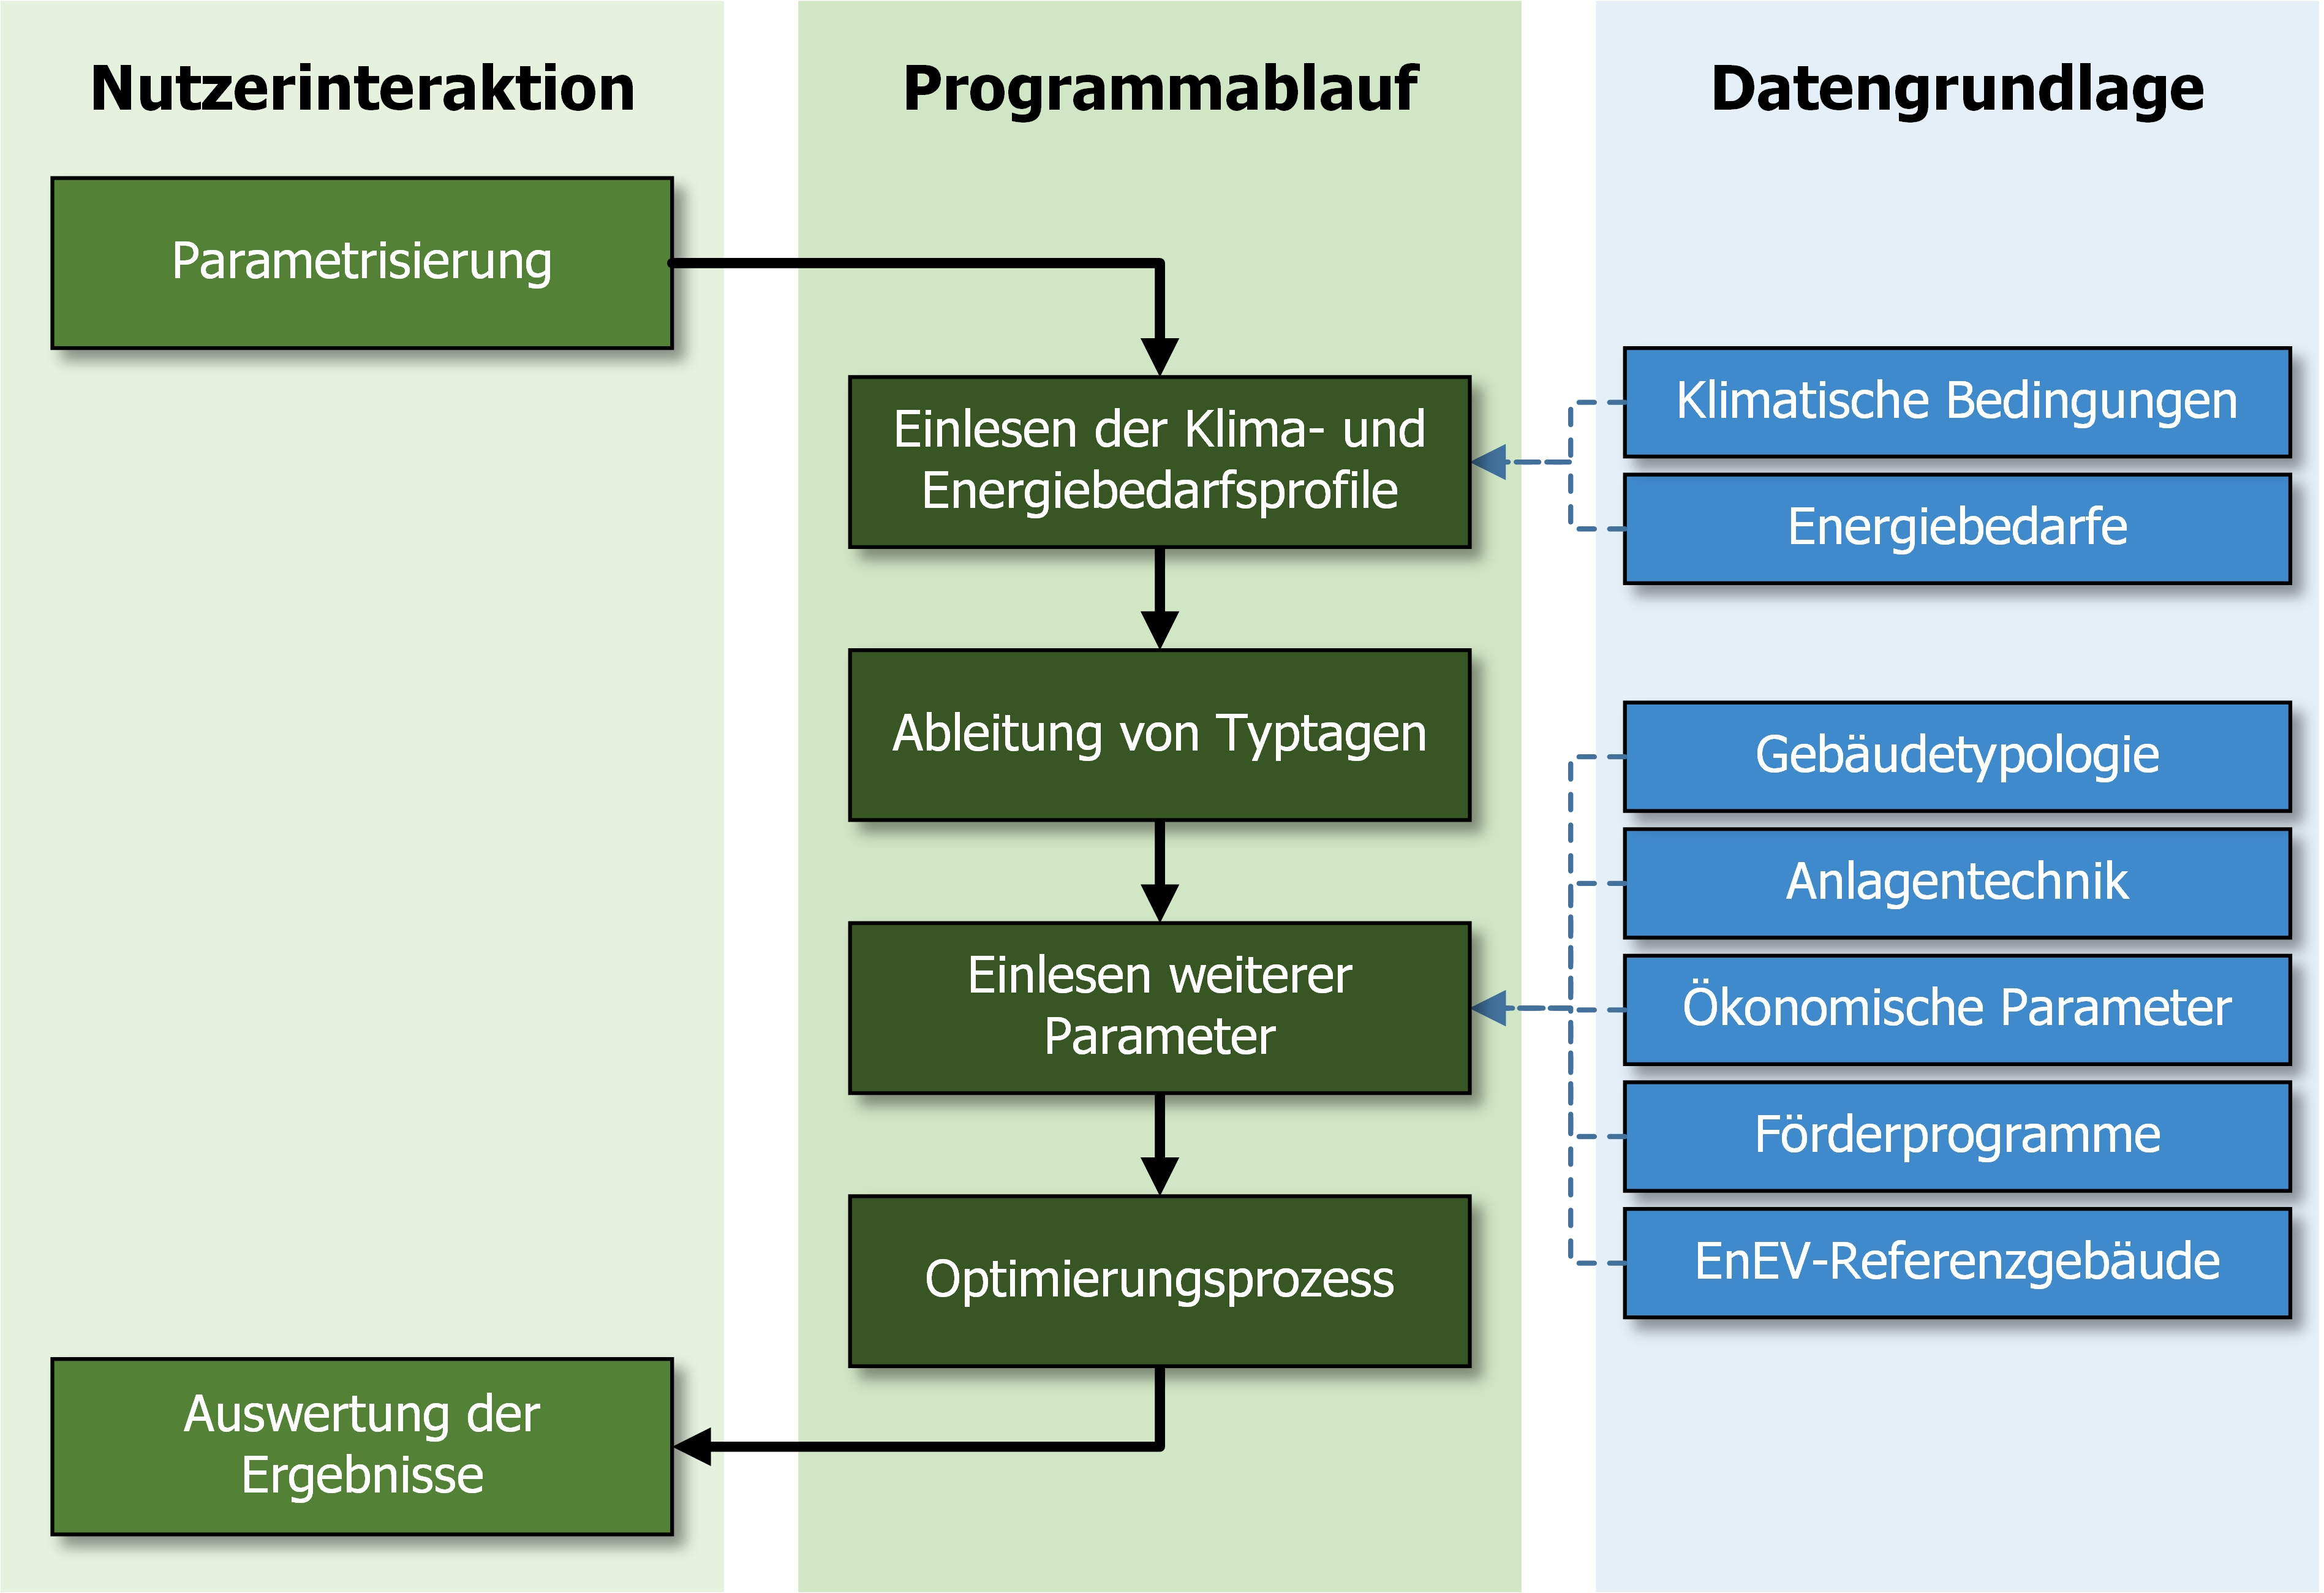
\includegraphics{Pictures/ProzessOptiProgramm.jpg}
	\caption{Schematischer Ablauf des Optimierungsprogrammes}
	\label{fig: Abbildung261} 
\end{figure}

\subsection{Parameteraufbereitung}
\label{subsec:Sektion261}

Zunächst werden dem Programm durch den Nutzer Angaben zum zu berechnenden Gebäude übergeben.
Hier werden Gebäudetyp, -alter und -lage sowie Wohnungsanzahl, Wohnfläche je Wohnung, Haushaltsgröße und qualitative Angaben zum Strom- und Trinkwarmwasserbedarfs definiert.
In Bezug auf den Gebäudetyp stehen die TABULA-Klassen Einfamilien-, Reihen-, Mehrfamilienhaus und Apartment-Block zur Wahl.
Auch die Baualtersklassen basieren auf TABULA-Unterteilungen und gliedern sich in 12 Klassen im Zeitraum von 1859 bis 2010.
Bei der Gebäudelage stehen dem Nutzer 15 verschiedene Städte aus verschiedenen Klimaregionen Deutschlands zur Auswahl.
Eine Übersicht über die möglichen Ausprägungen der Inputparameter Gebäudealter und -lage ist Tabelle \ref{tab: TabelleA3} zu entnehmen.

Auf Basis der übergebenen Angaben wird auf eine Datengrundlage zurückgegriffen.
So werden anhand des Gebäudestandortes entsprechende jährliche Klimaprofile genutzt.
Diese entsprechen dem Testreferenzjahr des Deutschen Wetterdienstes, welches für den Betrachtungszeitraum von 1981 bis 2010 einen repräsentativen Witterungsverlauf beschreibt.
Neben einem Umgebungstemperaturverlauf liefern die Profile solare Einstrahlungen und sind stündlich, also in 8760 Zeitpunkte, aufgeteilt.\\
Weiter werden Strom- und Trinkwarmwasserbedarfsprofile sowie Profile der internen Gewinne eingelesen.
Im Falle der Einfamilien- und Reihenhäuser hängen diese von der Haushaltsgröße ab und bei den Mehrfamilienhäusern sowie Apartment-Blocks von der Wohnungsanzahl.
Außerdem bedingen die Angaben zur Höhe des Strom- und Trinkwarmwasserbedarfes die Auswahl der Profile.
Die eingelesenen Verläufe basieren auf stochastischen Auswertungen des deutschen Stromspiegels und bilden Grundlasten sowie Lastspitzen ab.
Wie bei den Klimaprofilen sind auch diese als stündliche Werte über ein Jahr aufgetragen.

Da eine Optimierung über jede Stunde eines Jahres mit einem großen Rechenaufwand einhergeht, werden die eingelesenen Profile in Typtagen zusammengefasst. 
An Tagen mit vergleichbaren Witterungsverläufen ähneln sich die Energiebedarfsprofile, sodass diese im Rahmen des Programmes mit Hilfe eines Clusteringvorgangs zusammengefasst werden.
Um einerseits saisonale Effekte abzubilden und aussagekräftige Ergebnisse zu erhalten und andererseits die Rechenzeit des Programmes zu verkürzen, werden die 8760 Stunden eines Jahres in 8 Typtagen mit 192 Zeitpunkten zusammengefasst.
Diese besitzen wiederum Gewichtungen, welche in Summe 365 Tage und somit ein Jahr ergeben.

Neben den bereits erläuterten Klima- und Energiebedarfsprofilen werden weitere Gebäudeparameter an das Programm übergeben.
So werden für die Bauteile der Gebäudehülle U-Werte für drei Sanierungsszenarien eingelesen.
Bei diesen handelt es sich um den Standard-Zustand des parametrisierten Gebäudes im Bestand (standard), einer normalen energetischen Nachrüstung (retrofit) und außerdem einer fortgeschrittenen (advanced retrofit).
Zudem werden Faktoren zur Dimensionierung der Fenster-, Dach-, Boden- und Außenwandfläche eingelesen.
In Kapitel \ref{subsec:Sektion262} wird die Berechnung der Wärmeverluste anhand der U-Werte und der Bauteilflächen näher erläutert.
Schließlich werden auch ökonomische Faktoren zur Bestimmung des Preises einer Sanierungsmaßnahme in das Programm mit aufgenommen. 
Hierbei werden die Investitionskosten der Gebäudehüllenbestandteile als lineare Funktion ausgedrückt.
Außer bei den Fenstern berechnen sich diese Kosten anhand der zusätzlichen Dämmdicke im Zuge des Sanierungsszenario.
Im Falle der Verglasung wird die lineare Funktion anstelle der Dämmdicke in Abhängigkeit der Verbesserung des U-Wertes aufgestellt.
Die Werte für den y-Achsenabschnitt und die Steigung der linearen Funktionen für die einzelnen Bauteile basieren auf Berechnungen des IWU \cite{Hinz.10.08.2015} und sind in Tabelle \ref{tab: TabelleA4} aufgeführt.
Zusätzlich sind in dieser Tabelle Angaben zu der Nutzungsdauer der Komponenten zu finden, welche aus derselben Quelle entstammen.
Diese werden für die Berechnung der annualisierten Kosten benötigt.

Mit den bisher beschriebenen Daten lassen sich die Bedarfe des Gebäudes bestimmen.
Zur Deckung dieser werden verschiedene Energieerzeuger und -speicher zu dem Modell hinzugefügt.
Die Dimensionierung der jeweiligen Technologien erfolgt kontinuierlich.
Um die Investitionskosten der Anlagen zu berechnen, existieren Installationskosten für den Fall eines Einfamilienhauses oder Mehrfamilienhauses.
Zudem werden die Parameter einer linearen Funktion an das Programm übergeben oder anhand von Herstellerangaben durch das Modell generiert.
Tabelle \ref{tab: Tabelle2611} führt die verschiedenen Technologien, welche im Model Beachtung finden, sowie deren Nutzungsdauer auf.

\begin{table}[H]\centering
\begin{tabular}{|l|c|l|c|}
\hline
\rowcolor[HTML]{C0C0C0} 
Technologie     & \multicolumn{1}{l|}{\cellcolor[HTML]{C0C0C0}\begin{tabular}[c]{@{}l@{}}Nutzungsdauer\\ in Jahren\end{tabular}} & Technologie          & \multicolumn{1}{l|}{\cellcolor[HTML]{C0C0C0}\begin{tabular}[c]{@{}l@{}}Nutzungsdauer\\ in Jahren\end{tabular}} \\ \hline
\rowcolor[HTML]{EFEFEF} 
Brennwertkessel & 20                                                                                                             & Solarthermie         & 20                                                                                                             \\ \hline
Luft-Wärmepumpe & 18                                                                                                             & PV                   & 20                                                                                                             \\ \hline
\rowcolor[HTML]{EFEFEF} 
Sole-Wärmepumpe & 20                                                                                                             & Thermischer Speicher & 20                                                                                                             \\ \hline
\rowcolor[HTML]{EFEFEF} 
Pelletkessel    & 20                                                                                                             & Batteriespeicher     & 15                                                                                                             \\ \hline
\rowcolor[HTML]{EFEFEF} 
BHKW            & 15                                                                                                             & Elektroheizstab      & 20                                                                                                             \\ \hline
\end{tabular}
\caption{Anlagentechnik und deren Nutzungsdauer im Optimierungsmodell}
\label{tab: Tabelle2611}
\end{table}



%ökonomie
%Förderprogramme
%EnEV




\subsection{Optimierungsprozess}
\label{subsec:Sektion262}

Als Zielfunktion des Optimierungsprogrammes kann zwischen der Minimierung der annualisierten Kosten oder der CO\(_2\)-Emissionen ausgewählt werden.
Die Kosten setzten sich zusammen aus Investitionskosten durch die Anschaffung der Anlagentechnik und Verbesserung der Gebäudehülle (\(C_{Investition}\)), den Wartungs- und Instandhaltungskosten der Anlagen (\(C_{Variabel}\)), den Kosten aus dem Bedarf an Elektrizität und Brennstoffen (\(C_{Bedarf}\)), den Fixkosten durch Strom- und Gasbezug (\(C_{Fix}\)) sowie den Gewinnen aus dem Verkauf von Strom (\(R_{Erlöse}\)) und die Zuschüsse aus Fördergeldern (\(R_{Fördergelder}\)).
\begin{equation}
\label{eq:Gleichung2621}
C_{total} = \sum C_{Investition} + \sum C_{Variabel} + \sum C_{Bedarf} + \sum C_{Fix} - \sum R_{Erlöse} - \sum R_{Fördergelder}  
\end{equation}
Die Berechnung der Investitionskosten unterscheidet sich leicht zwischen Energieerzeugern und Hüllensanierung. 
Es ist zu erwähnen, dass das Standard-Szenario den Bestandszustand beschreibt und somit nicht mit Kosten verbunden ist.
Letztlich wird in allen Fällen eine totale Investitionssumme berechnet und unter Beachtung der jeweiligen Nutzungsdauer, dem internen Zinssatz und der Inflationsrate annualisiert.
Die betriebsgebundenen Kosten für Wartung und Instandhaltung werden anteilig aus den Investitionskosten bestimmt und mit einem Faktor zur Inflationsbereinigung beaufschlagt.
%weitere Kosten erläutern

Durch die Verbrennung von Brennstoffen wird CO\(_2\) freigesetzt. 
Somit kann die Emission beschrieben werden als Summe der CO\(_2\)-Freisetzung, die durch den Bedarf an Brennstoffe frei werden.
Hierbei ist noch zu beachten, dass sich die Emission durch Gutschriften aus Stromeinspeisungen in das Netz reduzieren lassen. %laut Norm?
Somit setzt sich die Berechnung der Emission aus der Verbrennung von Holz-Pellets (\(E_{Pellet}\)) oder Gas (\(E_{Gas}\)), dem Emissionswert des Stromes aus Netzbezug (\(E_{Netz}\)) und den negativen Emissionen der Gutschriften (\(E_{Einspeisung}\)) zusammen.
\begin{equation}
\label{eq:Gleichung2622}
E_{total} = E_{Pellet} + E_{Gas} + E_{Netz} - E_{Einspeisung}
\end{equation}
Die jeweiligen Summanden ergeben sich als Produkt aus dem Bedarf der Bezugsgröße und der leistungsspezifischen Emission der Emissionsquelle.
In Tabelle \ref{tab: Tabelle2621} sind die Werte für die Energiequellen Holz-Pellets, Gas und Strom aufgeführt.
Überschreitet die Elektrizitätsproduktion aus PV oder BHKW den Eigenbedarf des Gebäudes kann Strom ins Netz eingespeist werden, wodurch \(E_{Einspeisung}\) als Produkt der eingespeisten Energiemenge und dem leistungsspezifischen Emissionswert des Stromes berechnet wird.

\begin{table}[H]\centering
\begin{tabular}{|l|c|}
\hline
\rowcolor[HTML]{C0C0C0} 
Energiequelle                                                                                & \begin{tabular}[c]{@{}c@{}}CO\(_2\)-Emission\\ in {[}kg\(_{CO_2}\)/kWh{]}\end{tabular} \\ \hline
\rowcolor[HTML]{EFEFEF} 
Holz-Pellets                                                                          & 0,025                                                                        \\ \hline
Gas                                                                                   & 0,25                                                                         \\ \hline
\rowcolor[HTML]{EFEFEF} 
Strom                                                                                 & 0,566                                                                        \\ \hline
\end{tabular}
\caption{Leistungsspezifische Emission der Energieträger}
\label{tab: Tabelle2621}
\end{table}

Die Kombinationsmöglichkeiten zur Erfüllung der Zielfunktionen wird durch den Lösungraum, welcher durch Restriktionen definiert wird, beschränkt.
So wird beispielsweise die Anzahl der PV-Module durch die zur Verfügung stehende Dachfläche limitiert.
Eine zentrale Nebenbedingung stellt die Berechnung der Heizlast dar.
Diese beschreibt die Wärmemenge, welche durch die Anlagentechnik bereitgestellt werden muss, um das Gebäude auf die Norm-Innentemperatur in Höhe von 20\,°C zu heizen.
Als Berechnungsgrundlage dient die DIN EN 12831.
Diese definiert die Norm-Heizlast \(\Phi_{HL, build}\) als Summe der Transmissionswärmeverlusten \(\Phi_T\), Lüftungswärmeverlusten \(\Phi_{V, build}\), der Aufheizleistung \(\Phi_{hu}\) und abzüglich der internen Gewinne \(\Phi_{gain}\).
\begin{equation}
\label{eq:Gleichung2623}
\Phi_{HL, build} = \Phi_T + \Phi_{V, build} + \Phi_{hu} - \Phi_{gain}
\end{equation}
Die internen Gewinne werden aufgeteilt in solare Gewinne aus Sonneneinstrahlung und internen Wärmequellen wie beispielsweise Küchengeräte oder anwesende Personen.
Diese werden durch eingelesene Profile bestimmt und sind somit für das parametrisierte Gebäude für einen Zeitabschnitt konstant.
Da das Modell keine Gebäudemasse abbildet, kann die Aufheizleistung nicht berechnet werden.
Laut Norm ist \(\Phi_{hu}\) optional und wird somit vernachlässigt.

Die Transmissionswärmeverluste \(\Phi_T\) beschreiben Wärmeverluste aufgrund des Wärmeüberganges an der Gebäudehülle und lassen sich als Produkt der Temperaturdifferenz zwischen der Norm-Innentemperatur (\(\Theta_{int, i}\)) und der Außentemperatur (\(\Theta_e\)) mit dem Transmissionswärmetransferkoeffizienten (\(H_t\)) bestimmen und sind in Gleichung \ref{eq:Gleichung2624} wiedergegeben.
Letzterer wird als die Summe über die Bauteile der Produkte aus Bauteilfläche (\(A_k\)), U-Wert (\(U_k\)) und Temperaturkorrekturfaktor (\(f_{U,k}\)) ausgedrückt.
Außerdem werden Wärmebrücken mit dem zusätzlichen Wärmedurchgangskoeffizient (\(\Delta U_{TB}\)) berücksichtigt.
Die Formel zur Berechnung von \(H_t\) ist in \ref{eq:Gleichung2625} zu finden.
\begin{equation}
\label{eq:Gleichung2624}
\Phi_T = H_t \cdot (\Theta_{int, i} - \Theta_e)
\end{equation}
\begin{equation}
\label{eq:Gleichung2625}
H_t = \sum_{k} A_k \cdot (U_k + \Delta U_{TB}) \cdot f_{U,k} \qquad \text{mit k }\in \{\text{Außenwand, Boden, Fenster, Dach}\}
\end{equation}
Hierbei wird \(\Delta U_{TB}\) laut Norm vereinfacht mit 0,05 \(W/(m^2\cdot K)\) angenommen.
Der Temperaturkorrekturfaktor berücksichtigt einen Unterschied zwischen Norm-Innentemperatur und Außentemperatur.
Da in dem Programm keine Unterscheidung der Räume geschieht, gibt es nur im Falle des Bodens aufgrund des Kontaktes mit dem Erdreich einen solchen Unterschied.
Daher wird \(f_{U, Boden}\) nach Norm mit 0,6 bestimmt.
Die verschiedenen Kombinationsmöglichkeiten der Sanierungsszenarien werden durch Multiplikation mit einer binären Entscheidungsvariablen (\(x_{k, i}\)) in das Programm mit aufgenommen, wobei k \(\in\) \{Außenwand, Boden, Dach Fenster\} und i \(\in\) \{standard, retrofit, advanced retrofit\}.
\begin{equation}
\label{eq:Gleichung2626}
H_t = \sum_{k} \sum_{i} A_k \cdot (U_k + \Delta U_{TB}) \cdot f_{U,k} \cdot x_{k, i}
\end{equation}
Im Falle \(x_{k, i} = 1\), wird das Szenario gekauft und die Transmissionswärmeverluste werden gesenkt.
Analog hierzu entspricht \(x_{k, i} = 0\) einer Ablehnung für das Bauteil k das Szenario i zu kaufen.
Logischerweise können je Gebäudehüllenkomponente nicht mehr als eine Sanierungsmaßnahme vorgenommen werden, sodass das Modell durch die Nebenbedingung 
\begin{equation}
\label{eq:Gleichung2627}
\sum_{i} x_{k, i} = 1 \qquad \text{mit i } \in \{\text{standard, retrofit, advanced retrofit}\}
\end{equation}
beschränkt wird.

Schließlich wird die Heizlast auch durch die Lüftungswärmeverluste beeinflusst.
Diese werden durch das Heizperiodenverfahren in DIN V 4108-6 modelliert.
Hierzu wird laut Norm von einer Luftwechselrate (n) für ein nicht luftdichtheitsgeprüftes Gebäude von 0,7\,h\(^{-1}\) ausgegangen. 
Die Luftwechselrate beschreibt, wie oft pro Stunde das Volumen des Gebäudes mit Frischlust ausgetauscht wird.
Des Weiteren wird das Netto-Volumen (V) in der Norm als 0,76-fachen des Brutto-Volumens (V\(_e\)) bestimmt.
Somit ergibt sich mit der Wärmekapazität der Luft (c\(_{p, Luft}\)) und der Luftdichte (\(\rho_{Luft}\)) die spezifische Lüftungswärmeverluste (\(H_V\)) zu
\begin{equation}
\label{eq:Gleichung2628}
H_V = 0,76 \cdot V_e \cdot \rho_{Luft} \cdot c_{p, Luft} \cdot n \quad \text{.}
\end{equation}
Zuletzt wird durch Berücksichtigung des Korrekturfaktor aufgrund von Nachtabschaltung der Heizung (f\(_{NA} = 0,95\)) und des Gradtagzahlfaktor (G\(_t\)) die Lüftungswärmeverluste zu
\begin{equation}
\label{eq:Gleichung2629}
\Phi_{V, build} = H_V \cdot G_t \cdot f_{NA} \cdot 24 \frac{h}{d} \cdot \frac{1}{1000} \frac{kW}{W} 
\end{equation}
berechnet.
